\chapter{Desarrollo}
\label{cha:development}

En esta sección se expone el análisis de la aplicación web Ruby on Rails, de 3 capas, utilizada para el desarrollo del proyecto. Además, se detallan las decisiones de diseño y desarrollo de cada una de las iteraciones a realizar a partir de la misma.

\section{Análisis de la aplicación Ruby on Rails}

La aplicación \kode{sample\_app\_rails\_4}, escrita en lenguaje Ruby\footnotettt{Ruby}{https://www.ruby-lang.org/es}, es parte de un tutorial sobre el uso del \textit{framework} de desarrollo de aplicaciones web Ruby on Rails\footnotettt{Ruby on Rails}{http://www.rubyonrails.org.es}. Se trata de una aplicación de muestra, desarrollada mediante una combinación de simulaciones, pruebas de desarrollo \textit{TDD} y pruebas de integración. Tiene una arquitectura de 3 capas: cliente, aplicación y base de datos. Está creada a partir de páginas estáticas con contenido dinámico, tiene un diseño de sitio web, un modelo de datos de usuario y un sistema completo de registro y autenticación, incluida la activación de cuentas y restablecimientos de contraseñas. Además tiene funciones de \textit{microblogging} y redes sociales. Así, tendrá usuarios que crearán \textit{microposts} dentro de un marco de autenticación e inicio de sesión completo.

\begin{figure}[H]
\image{images/figures/sampleapp.png}
\caption{Integración entre características y componentes de Ruby on Rails.}
\end{figure}

La arquitectura de Ruby on Rails que implementa la aplicación web tiene las siguientes características:
\begin{itemize}
\item Arquitectura Modelo-Vista-Controlador (MVC): Mejora la capacidad de mantenimiento, desacoplamiento y pruebas de la aplicación.
\item Arquitectura \textit{Representational State Transfer} (REST) para servicios web.
\item Soporta las principales bases de datos como MySQL\footnotettt{MySQL}{https://www.mysql.com}, Oracle\footnotettt{Oracle}{https://www.oracle.com/es/database/index.html} y PostgreSQL\footnotettt{PostgreSQL}{http://www.postgresql.org.es}, entre otras.
\item Lenguaje \textit{scripting} del lado del servidor de código abierto.
\item Convención sobre configuración.
\item Generadores de \textit{scripts} para automatizar tareas.
\item Uso de \textit{YAML}, formato de serialización de datos inspirado en lenguajes como \textit{XML} y \textit{C}.
\end{itemize}

Las características anteriormente descritas se distribuyen en los siguientes componentes de Rails:
\begin{itemize}
\item \textit{Action Mailer}: Proporciona servicios de correo electrónico. 
\item \textit{Action Pack}: Capta las solicitudes de usuario realizadas por el navegador y las asigna a acciones definidas en la capa de controladores.
\subitem-- \textit{Action Controller}: Enruta solicitudes a su controlador correspondiente. 
\subitem-- \textit{Action Dispatcher}: Controla, analiza y procesa el enrutamiento de la solicitud del navegador web.
\subitem-- \textit{Action View}: Realiza la presentación de la página web solicitada.
\item \textit{Active Model}: Define la interfaz entre el \textit{Action Pack} y los módulos \textit{Active Record}.
\item \textit{Active Record}: Proporciona capacidad de crear relaciones o asociaciones entre modelos y construye la capa Modelo que conecta las tablas de la base de datos con su representación en las clases Ruby.
\item \textit{Active Resource}: Administra la conexión entre servicios web \textit{RESTful} y objetos de negocio.
\item \textit{Active Support}: Colección de clases de utilidad y extensiones de bibliotecas estándar de Ruby útiles para el desarrollo en Ruby on Rails.
\item \textit{Railties}: Código básico de Rails que construye nuevas aplicaciones. 
\end{itemize}	 

\begin{figure}[H]
\centering
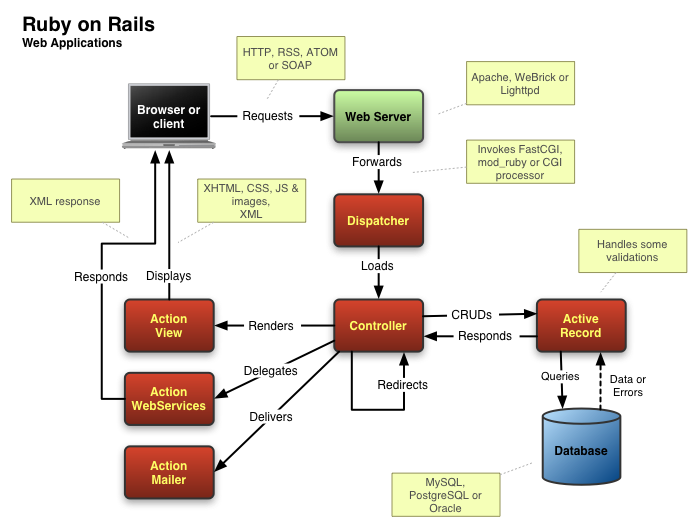
\includegraphics[width=0.7\textwidth]{images/figures/rubyonrails.png}
\caption{Integración entre características y componentes de Ruby on Rails.}
\end{figure}

Una vez vistas las características y capacidades, tanto de una aplicación Ruby on Rails genérica como de la aplicación en actual estudio, se decide elaborar un trabajo adicional sobre ella, aplicando una serie de cambios y adiciones para la consecusión de los objetivos propuestos, inicialmente.

\section{Iteración 1: Conversión a una arquitectura de microservicios con el uso de Docker}

La primera iteración del proyecto consiste en adecuar la aplicación Ruby on Rails para que utilice contenedores en su funcionamiento. Esta tarea supone su despliegue en una sola máquina física.

La aplicación \kode{sample\_app\_rails\_4} está disponible en un repositorio GitHub. Para trabajar con ella se hace una copia del repositorio a través de un \textit{fork}. Esto crea una bifurcación que permite la libre experimentación de cambios, sin afectar el proyecto original, utilizando el proyecto de otra persona como punto de partida de una idea propia.

Una vez se tiene una copia local y se comprueba que funciona correctamente se va a hacer uso de la tecnología de contenerización Docker para desplegar la siguiente estructura:

\begin{figure}[H]
\image{images/figures/iteration1.png}
\caption{Estructura del despliegue monomáquina con contenedores Docker.\label{fig:figure_docker_microservices}}
\end{figure}

Mediante Docker se obtienen las imágenes pertenecientes a dos servicios. El primero implementa la funcionalidad de la base de datos \kode{PostgreSQL} y el segundo implementa el servidor web y proxy inverso \kode{Nginx}. El proxy inverso es un proxy que aparenta ser un servidor web ante los clientes, pero que en realidad reenvía las solicitudes que recibe a uno o más servidores de origen. Se escoge \kode{Nginx} por ser multiplataforma, ligero, de alto rendimiento y software libre.

La aplicación en su origen utiliza una base de datos \kode{SQLite}\footnotettt{SQLite}{https://sqlite.org} que va a ser cambiada por la base de datos \kode{PostgreSQL}, provisionada por el contenedor \kode{some-postgres}. 

Otro de los cambios a implementar es la sustitución del servidor web \kode{rails s} por \kode{puma}\footnotettt{Servidor Web Puma}{http://puma.io}, construido para ofrecer mayor velocidad y paralelismo.

Como se ha comentado, a través de Docker se pueden obtener las imágenes de los servidores \kode{PostgreSQL} y \kode{Nginx}, pero para poder crear un contenedor que contenga la aplicación web habrá que crear su imagen Docker. 

El principal propósito de este despliegue es que pueda realizarse automáticamente tras la ejecución de un \textit{script}. Este fichero comprobará que las variables de entorno que especifican el nombre y la contraseña del usuario de las distintas bases de datos PostgreSQL existentes (test, desarrollo y producción) están correctamente establecidas.

La siguiente acción a realizar será la construcción de la imagen Docker de la aplicación web, que se llamará \kode{sample\_app\_rails\_4\_image}. 

Luego se creará el contenedor \kode{some-postgres} con el servidor \kode{PostgreSQL} y, seguidamente, se creará el contenedor de la aplicación web, llamado \kode{some-app}, a partir de la imagen de ésta, enlazándola con el contenedor \kode{some-postgres}, que será su base de datos.

Con la intención de utilizar como servidor web de la aplicación un contenedor diferente al propio, se crea el contenedor \kode{some-nginx} que proporciona el servidor \kode{Nginx}. Se le indicará que el tráfico del puerto 8080 en el sistema anfitrión se redirija al 80 del contenedor. Así, el sitio web será accesible por la dirección local en el puerto 8080. Además, se enlazará a la aplicación web mediante el contenedor en el que se ejecuta, y se montará el volumen Docker compartido \kode{volume-public}.

Así, solo quedará construir, migrar y poblar la base de datos que se ejecuta en el contenedor \kode{some-app}, dentro del contenedor \kode{some-postgres}.

Finalmente, se ejecutará el servidor \kode{puma} dentro del contenedor \kode{some-app} y se comprobará desde el sistema anfitrión que la página principal de la aplicación \kode{sample\_app\_rails\_4} está disponible en el puerto 8080. Esto producirá el siguiente resultado:

\begin{figure}[H]
\centering
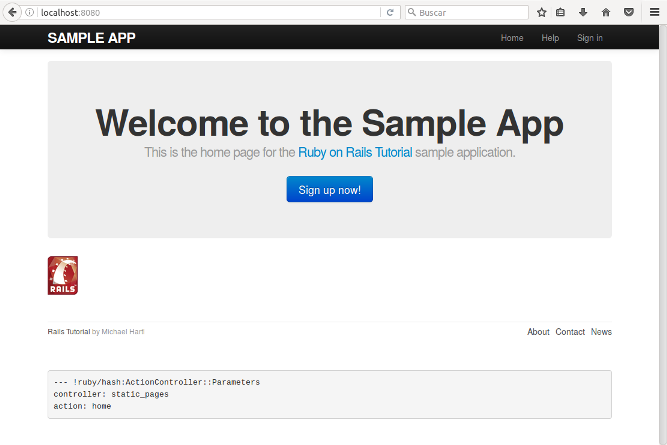
\includegraphics[width=0.7\textwidth]{images/figures/resultado1.png}
\caption{Resultado de la Iteración 1 con el uso de Docker.}
\end{figure}

A efectos de mantener la imagen de la aplicación remotamente se subirá al repositorio DockerHub con la etiqueta \kode{initial}.

\subsection{Preparación del repositorio local y remoto}

En primer lugar se realiza una copia del repositorio GitHub de la aplicación \kode{sample\_app\_rails\_4}. Para ello se realiza un \textit{fork} seleccionando el botón con el mismo nombre y automáticamente se crea la copia del repositorio en la cuenta personal. Seguidamente se clona esta copia para trabajar localmente:

%= lang:bash
\begin{code}
$ git clone https://github.com/CarolinaSantana/sample_app_rails_4-1.git 
\end{code}

Luego se entra en la carpeta local que lo contiene, seleccionando como \textit{gemset}, conjunto aislado de gemas incorporadas en la aplicación para la versión Ruby en uso, 2.0.0, quedando como \kode{2.0.0@railstutorial\_rails\_4\_0}. Además se deja lista la configuración de base de datos, utilizando la que viene a modo de ejemplo, con la intención de probar que los test que comprueban su funcionalidad pasen positivamente: 

%= lang:bash
\begin{code}
$ cd sample_app_rails_4-1
$ cp config/database.yml.example config/database.yml
$ bundle install --without production
$ bundle exec rake db:migrate
$ bundle exec rake db:test:prepare
$ bundle exec rspec spec/
\end{code}

\subsection{Cambio y configuración de la base de datos} \label{postgrescredentials}

Con la intención de implementar la base de datos de la aplicación desde un contenedor Docker se elimina del fichero \kode{Gemfile} la gema \kode{sqlite3 1.3.8}, como base de datos en desarrollo, y se cambia por una base de datos PosgreSQL, concretamente la versión \kode{pg 0.15.1}. Para instalar la nueva gema se ejecuta:

%= lang:bash
\begin{code}
$ bundle install --without production
\end{code}

La instalación de \kode{PostgreSQL} requiere credenciales de usuario con contraseña para acceder. La manera de especificarlo es mediante las variables de entorno \kode{\$POSTGRES\_USER} y \kode{\$POSTGRES\_PASSWORD} en el fichero local \kode{\textasciitilde{}/.postgres/credentials} cuyo contenido es:

\begin{codelisting}
\label{code:credentials}
\codecaption{Fichero \kode{\textasciitilde{}/.postgres/credentials}}
\begin{code}
export POSTGRES_USER=postgres
export POSTGRES_PASSWORD=postgres
\end{code}
\end{codelisting}

Se da permiso de ejecución tanto al fichero como a la carpeta que lo contiene y se exportan las variables de entorno en el directorio de la aplicación:

%= lang:bash
\begin{code}
$ chmod 0700 ~/.postgres
$ chmod 0700 ~/.postgres/credentials
$ . ~/.postgres/credentials
\end{code}

Ahora se cambia el fichero de configuración de la base de datos de forma que se especifique lo siguiente:

\begin{codelisting}
\label{code:database}
\codecaption{Cambios en el fichero \kode{config/database.yml}}
\begin{code}
default: &default
  adapter: postgresql
  encoding: unicode
  pool: 5
  username: <%= ENV['POSTGRES_USER'] %>
  password: <%= ENV['POSTGRES_PASSWORD'] %>
  port: 5432
development:
  <<: *default
  database: sample_app_development  
  host : db
test:
  <<: *default
  database: sample_app_test
  host: db
production:
  <<: *default
  database: sample_app_production
\end{code}
\end{codelisting}

Así, se ha indicado a las bases de datos de desarrollo, test y producción el nombre de usuario y contraseña, a partir de variables de entorno. Además, se especifica que ha de conectarse a \textit{db}, que será el nombre por el que ha de descubrir el contenedor docker que provisiona el servidor \kode{PostgreSQL}.

Por motivos de seguridad el fichero de configuración de la base de datos no se ha de subir al repositorio remoto, por lo que se hace una copia para tener esta configuración de ejemplo:

%= lang:bash
\begin{code}
$ cp config/database.yml config/database.yml.postgres
\end{code}

\subsection{Creación de un alimentador de base de datos idempotente}

Con la intención de que cuando ya existan datos en la base de datos no se vuelvan a crear, se cambia el fichero \kode{lib/tasks/sample\_data.rake}, que viene por defecto, para que sea un \textit{seed} idempotente. Solo se crearán datos en la base de datos si aún no existen, quedando el fichero como:

\begin{codelisting}
\label{code:idempotentseed}
\codecaption{Fichero \kode{lib/tasks/sample\_data.rake}}
%= lang:ruby
\begin{code}
namespace :db do
  desc "Fill database with sample data"
  task populate: :environment do
    make_users_microposts_relationships
  end
end
def make_users_microposts_relationships
  User.find_or_create_by(email:"example@railstutorial.org") do |admin| 
  	admin.name = "Example User"
	admin.password = "foobar"
        admin.password_confirmation = "foobar"
        admin.admin = true
	99.times do |n|
	    name  = Faker::Name.name
	    email = "example-#{n+1}@railstutorial.org"
	    password  = "password"
	    User.create!(name:     name,
                 email:    email,
                 password: password,
                 password_confirmation: password)
        end
	users = User.all(limit: 6)
  	50.times do
	    content = Faker::Lorem.sentence(5)
	    users.each { |user| user.microposts.create!(content: content) }
	end  
	users = User.all
	user  = users.first
	followed_users = users[2..50]
	followers      = users[3..40]
	followed_users.each { |followed| user.follow!(followed) }
	followers.each      { |follower| follower.follow!(user) }
  end
end
\end{code}
\end{codelisting}

\subsection{Cambio y configuración del servidor web}

Por su parte, para poder acceder a la aplicación en cuestión, se cambia el servidor web \kode{rails s} por \kode{puma}\footnotettt{Servidor Web Puma}{http://puma.io}. Para ello se añade al fichero \kode{Gemfile} la siguiente entrada:

\begin{codelisting}
\label{code:addpuma}
\codecaption{Fichero \kode{Gemfile}}
%= lang:ruby
\begin{code}
.
gem 'puma'
.
\end{code}
\end{codelisting}

Luego se instala la nueva gema: 

%= lang:bash
\begin{code}
$ bundle install --without production
\end{code}

\subsection{Configuración automatizada para la creación de los contenedores}

En primer lugar se configuran los registros o \textit{logs} que crearán los contenedores añadiendo en el fichero \kode{config/application.rb} lo siguiente:

\begin{codelisting}
\label{code:application.rb}
\codecaption{Fichero \kode{config/application.rb}}
%= lang:ruby
\begin{code}
.
config.logger = Logger.new(STDOUT)
.
\end{code}
\end{codelisting}

Además, se añade el fichero \kode{.dockerignore} para que la imagen Docker del repositorio que se construya sea más ligera:

\begin{codelisting}
\label{code:.dockerignore}
\codecaption{Fichero \kode{.dockerignore}}
%= lang:ruby
\begin{code}
.
cp .gitignore .dockerignore
.
\end{code}
\end{codelisting}

En este momento ya se tienen listas las configuraciones necesarias para proceder a la creación de los contenedores. Para ello se comienza a ejecutar el script \kode{docker-microservice.sh}.

En primer lugar, se comprueba que las variables de entorno que especifican el nombre y la contraseña del usuario de la base de datos PostgreSQL están establecidas.

Para crear el contenedor de la aplicación primero se construye su imagen, que se llamará \kode{sample\_app\_rails\_4\_image}. Así, es necesario crear un fichero \kode{Dockerfile} que especifica cómo crearla, indicando que lo hará a partir de una imagen Ruby y que debe actualizar todos los paquetes e instalar \textit{nodejs}, requerido por la aplicación, y la utilidad netcat, para comprobar que el servicio PostgreSQL está listo. Tras ello se le indica que haga una limpieza de las capas intermedias. 

La lógica de construcción de la aplicación basada en su imagen pasa por la creación de dos contenedores. El primer contenedor, \kode{app-job}, se configurará a partir de un \textit{entrypoint} que permite ejecutar un contenedor como un ejecutable. Este contenedor esperará a que el servicio \textit{PostgreSQL} esté activo en el contenedor \kode{some-postgres} para crear, migrar, alimentar y poblar las bases de datos. Una vez acaba el contenedor también termina. Para poder especificar el \textit{entrypoint} es necesario copiar el fichero script \kode{setup.sh}, que se encarga de ello, dentro del contenedor, indicando la copia en \kode{Dockerfile}. 

\begin{codelisting}
\label{code:dockerfile}
\codecaption{Fichero \kode{setup.sh}}
%= lang:ruby
\begin{code}
#!/bin/sh

cp config/database.yml.postgresql config/database.yml
echo "Waiting PostgreSQL to start on 5432..."
while ! nc -z some-postgres 5432; do
  sleep 0.1
done
echo "PostgreSQL started"
echo "Creating databases..."
rake db:create
echo "Migrating to databases..."
rake db:migrate
echo "Seeding databases..."
rake db:seed
echo "Populating databases..."
rake db:populate
echo "Ready databases"
\end{code}
\end{codelisting}

Así como se tiene el contenedor \textit{job} se necesita un segundo contenedor \textit{task}, concretamente llamado \kode{app-task}. Este contenedor se construye a partir del anterior.

\begin{codelisting}
\label{code:dockerfile}
\codecaption{Contenido de \kode{Dockerfile}}
%= lang:ruby
\begin{code}
FROM ruby:2.0-onbuild
LABEL sample_app_rails_4_image.version="0.1" 
      sample_app_rails_4_image.release-date="2016-12-10"
MAINTAINER Carolina Santana "c.santanamartel@gmail.com"
RUN apt-get update && apt-get -y install nodejs && \
    apt-get -y install netcat && \
    apt-get autoclean && apt-get clean && \
    rm -rf /var/lib/apt/lists/* && \
    rm -f /tmp/* /var/tmp/*
COPY /setup.sh /
\end{code}
\end{codelisting}

La siguiente acción es la creación del contenedor \kode{some-postgres} con el servidor \kode{PostgreSQL}, a partir de la imagen \kode{postgres} indicada con \textit{\--d}. Para poder acceder a la base de datos es necesario pasarle las credenciales, con \textit{\--e}. 

Con la intención de exportar un volumen compartido entre los contenedores \kode{app-task} y \kode{some-nginx} para que compartan el directorio \kode{/usr/src/app/public} y el directorio \kode{/var/lib/postgresql} con el contenedor \kode{some-postgres} se crea un volumen Docker llamado \kode{volume-public}.

Ahora se crea el contenedor \textit{job} de la aplicación web, llamado \kode{app-job}, a partir de la imagen de ésta, \textit{\--d}, indicando como \textit{\---entrypoint} el script comentado, enlazando la base de datos de la misma con el contenedor \kode{some-postgres} a través del indicador \textit{\--link}. Además, se le pasan las variables de entorno necesarias para acceder a la base de datos, con \textit{\--e}. Por su parte, el indicador \textit{\--it} ofrece un terminal interactivo dentro del contedor y \textit{\--w} indica que se va a compartir el directorio inicial del proyecto local en el contenedor. El volumen creado se exporta mediante \textit{\--v}.

El siguiente paso crea el contenedor \textit{task} de la aplicación web, llamado \kode{app-task}. Este se construye como el anterior obviando el paso del \textit{entrypoint}. Además, se configuran y preparan las bases de datos, así como se ejecuta el servidor \kode{puma} en el puerto \kode{9292} para que la aplicación pueda ser accesible, todo ello a través de \textit{/bin/bash \--c}

Para crear el contenedor \kode{some-nginx} que proporciona el servidor \kode{Nginx} se indica la imagen con \textit{\--d}, que el tráfico del puerto 8080 en el sistema anfitrión se redirija al 80 del contenedor, \textit{\--p}, y se enlaza la aplicación web con el contenedor en el que se ejecuta, a través del indicador \textit{\--link}. Además se monta el volumen \kode{volume-public} con el indicador \textit{\--v}. Por último, se crea localmente el fichero de configuración \kode{/etc/nginx/conf.d/nginx.conf} en el que se especifica que este servidor escuchará en el puerto 80, compartiendo el directorio \kode{/usr/src/app/public}, también indicado en la creación con \textit{\--w}, así como que ha de resolver la aplicación en el puerto 9292, que es el que usa \kode{puma} para la ejecución.  

El contenido de este fichero es: 
\begin{codelisting}
\label{code:nginxconf}
\codecaption{Contenido de \kode{nginx.conf}}
%= lang:java
\begin{code}
server {
  listen 80;
  root /usr/src/app/public;
  location / {
    proxy_set_header X-Forwarded-For $proxy_add_x_forwarded_for;
    proxy_set_header Host $http_host;
    proxy_redirect off;
    try_files $uri /page_cache/$uri /page_cache/$uri.html @app;
  }
  location @app{
    proxy_pass http://app:9292;
    break;
  }
}
\end{code}
\end{codelisting}

Así, se accede al contenedor \kode{some-app} para poder construir, migrar y poblar la base de datos que se ejecuta en el contenedor \kode{some-app}, dentro del contenedor \kode{some-postgres}.

El script utilizado, con permiso \kode{chmod +x} y ejecutado como \kode{./docker-microservices.sh}, es el siguiente:

\begin{codelisting}
\label{code:scriptdocker}
\codecaption{Contenido de \kode{docker-microservices.sh}}
%= lang:bash
\begin{code}
#!/bin/bash

if [ "$POSTGRES_USER" = "" ] || [ "$POSTGRES_PASSWORD" = "" ]; then
	echo "Environment variables for POSTGRES not found"
        exit
fi
docker build -t sample_app_rails_4_image .
docker run --name some-postgres -e POSTGRES_USER=$POSTGRES_USER \
  -e POSTGRES_PASSWORD=$POSTGRES_PASSWORD -d postgres
docker volume create --name volume-public
docker run -i --name app-job --entrypoint /setup.sh \
  -e POSTGRES_USER=$POSTGRES_USER -e POSTGRES_PASSWORD=$POSTGRES_PASSWORD \
  -w /usr/src/app -v volume-public:/var/lib/postgresql \
  --link some-postgres:db sample_app_rails_4_image
docker run -d -it --name app-task -e POSTGRES_USER=$POSTGRES_USER \
  -e POSTGRES_PASSWORD=$POSTGRES_PASSWORD -w /usr/src/app \
  -v volume-public:/usr/src/app/public --link some-postgres:db \
  sample_app_rails_4_image \
  /bin/bash -c "cp config/database.yml.postgresql config/database.yml \
                && puma -p 9292"
docker run --name some-nginx \
  -v "${PWD}/nginx.conf":/etc/nginx/conf.d/default.conf \
  -p 8080:80 --link app-task:app -v volume-public:/usr/src/app/public -d nginx
\end{code}
\end{codelisting}

\subsection{Resultado}

El resultado del script anterior crea los distintos elementos propuestos en el planteamiento de esta iteración. Así las imagenes Docker descargadas y la creada, perteneciente a la aplicación, son:

\begin{figure}[H]
\centering
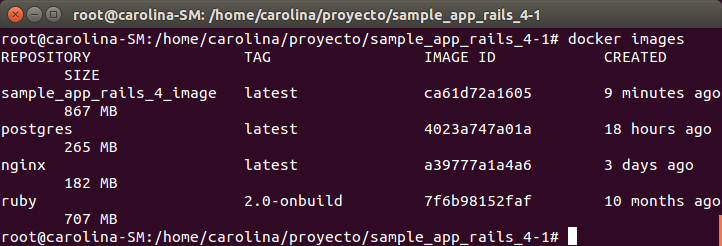
\includegraphics[width=0.8\textwidth]{images/figures/dockerimages.png}
\caption{Imágenes docker mostradas con \kode{docker images}.}
\end{figure}

Y los contenedores Docker creados son:

\begin{figure}[H]
\centering
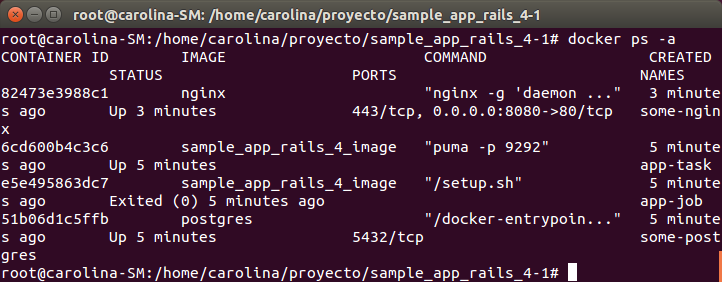
\includegraphics[width=0.8\textwidth]{images/figures/dockerps.png}
\caption{Contenedores docker mostrados con \kode{docker ps -a}.}
\end{figure}

De esta manera, en el contenedor \kode{app-task} se encuentra en ejecución el servidor \kode{puma}, así que se puede comprobar desde el sistema anfitrión que la página principal de la aplicación \kode{sample\_app\_rails\_4} está disponible en el puerto 8080, mediante el comando \kode{curl http://localhost:8080}:

\begin{figure}[H]
\centering
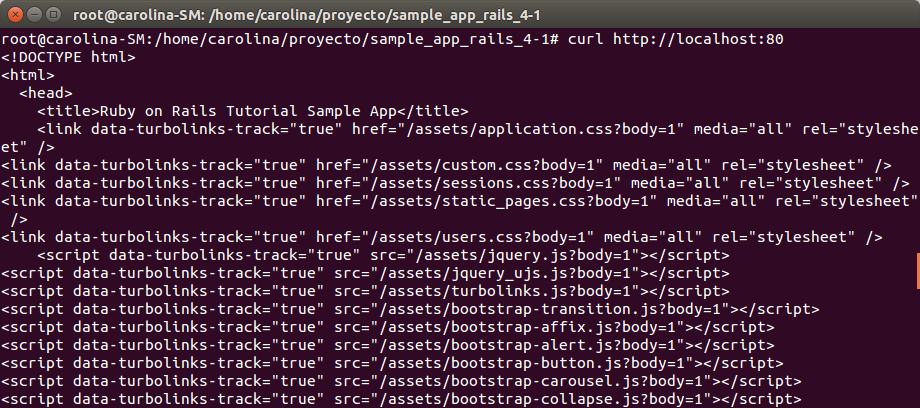
\includegraphics[width=0.8\textwidth]{images/figures/curldocker.png}
\caption{Volcado de ejecución \kode{curl http://localhost:8080}.}
\end{figure}

Así, a partir de ahora se podrá hacer el despliegue partiendo de la imagen local. Para poder hacerlo de forma automatizada se crea el fichero \kode{docker-microservices-deploy.sh}, con permiso \kode{chmod +x} y ejecutado como \kode{./docker-microservices.sh}, es el siguiente:

\begin{codelisting}
\label{code:scriptdocker}
\codecaption{Contenido de \kode{docker-microservices-deploy.sh}}
%= lang:bash
\begin{code}
#!/bin/bash

if [ "$POSTGRES_USER" = "" ] || [ "$POSTGRES_PASSWORD" = "" ]; then
	echo "Environment variables for POSTGRES not found"
        exit
fi
docker run --name some-postgres -e POSTGRES_USER=$POSTGRES_USER \
  -e POSTGRES_PASSWORD=$POSTGRES_PASSWORD -d postgres
docker volume create --name volume-public
docker run -i --name app-job --entrypoint /setup.sh \
  -e POSTGRES_USER=$POSTGRES_USER \
  -e POSTGRES_PASSWORD=$POSTGRES_PASSWORD -w /usr/src/app \
  -v volume-public:/var/lib/postgresql --link some-postgres:db \
  carolina/sample_app_rails_4_image:latest
docker run -d -it --name app-task -e POSTGRES_USER=$POSTGRES_USER \
  -e POSTGRES_PASSWORD=$POSTGRES_PASSWORD -w /usr/src/app \
  -v volume-public:/usr/src/app/public --link some-postgres:db \
  carolina/sample_app_rails_4_image:latest \
  /bin/bash -c "cp config/database.yml.postgresql config/database.yml \
                && puma -p 9292"
docker run --name some-nginx \
  -v "${PWD}/nginx.conf":/etc/nginx/conf.d/default.conf \
  -p 8080:80 --link app-task:app -v volume-public:/usr/src/app/public -d nginx
\end{code}
\end{codelisting}

De esta forma, este despliegue operará y ofrecerá los servicios de la misma manera que el anterior.

\section{Iteración 2: Subida de la imagen resultante de la aplicación al repositorio de imágenes DockerHub}

A efectos de mantener la imagen remotamente se sube al repositorio DockerHub, previa creación de una cuenta en él. Para ello se inicia sesión por consola y se añade una etiqueta a la imagen \kode{sample\_app\_rails\_4\_image}, especificando su identificador y el repositorio escogido dentro de la cuenta:

%= lang:bash
\begin{code}
$ docker login
$ docker tag <image-id> carolina/sample_app_rails_4_image:initial
$ sudo docker push carolina/sample_app_rails_4_image
\end{code}

Cuando se muestran las imágenes docker se aprecia la etiquetación hecha:

\begin{figure}[H]
\centering
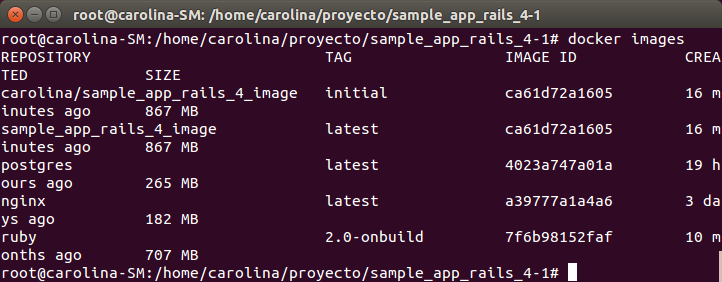
\includegraphics[width=0.8\textwidth]{images/figures/dockerimages2.png}
\caption{Imágenes docker mostradas con \kode{docker images}.}
\end{figure}

La subida de la imagen etiquetada como \kode{initial} se puede apreciar ahora en Docker Hub:

\begin{figure}[H]
\centering
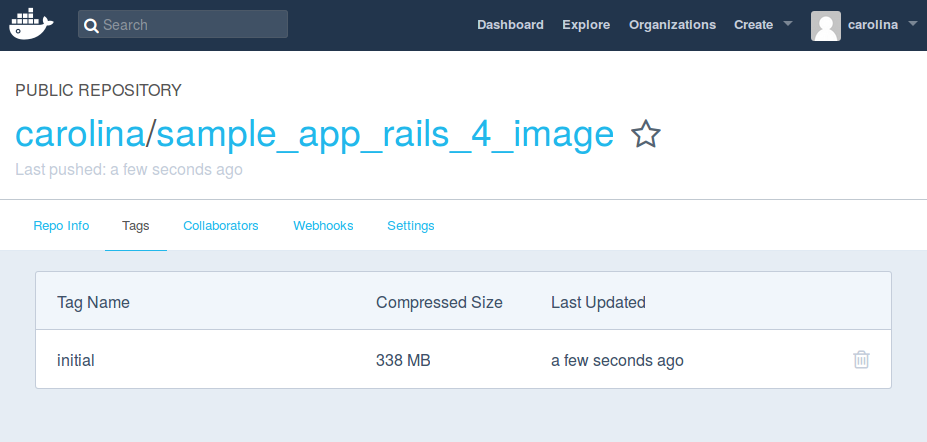
\includegraphics[width=0.8\textwidth]{images/figures/dockerhubinitial.png}
\caption{Imágenes docker mostradas con \kode{docker images}.}
\end{figure}

También puede ser comprobado localmente mediante:

%= lang:bash
\begin{code}
$ docker images carolina/sample_app_rails_4_image:initial
\end{code}

Cuyo resultado es:

\begin{figure}[H]
\image{images/figures/dockerimages3.png}
\caption{Resultado de la búsqueda de la imagen con \kode{docker search}.}
\end{figure}

\section{Iteración 3: Integración y Despliegue continuos de la aplicación con Travis CI y GitHub}

En esta iteración se busca adaptar la aplicación Ruby on Rails para que funcione con Travis CI. Esta herramienta se conectará al repositorio de GitHub \kode{sample\_app\_rails\_4-1} con la intención de poder generar una imagen Docker de la aplicación tras cada cambio. Esto permite trabajar en un entorno de desarrollo en el que la integración de los cambios en el proyecto es continua, así como también su despliegue es automatizado.

Para ello se realiza el siguiente proceso:
\begin{figure}[H]
\image{images/figures/iteration2.png}
\caption{Integración y Despliegue continuos con Travis CI.}
\end{figure}

Las precondiciones, condiciones y postcondiciones necesarias para construir y desplegar la aplicación en uso de manera automática se especifican en el fichero \kode{.travis.yml}. A este fichero se le añadirán, además, las credenciales de la cuenta de DockerHub mediante variables de entorno encriptadas, sumando una respectiva al repositorio GitHub. Las acciones a realizar serán la comprobación de que los tests pasan satisfactoriamente, la construcción de una nueva imagen Docker y su subida al repositorio DockerHub.

Para llevarlo a cabo es necesario añadir una configuración de base de datos específica. En este caso se llamará \kode{travis\_ci\_test}.

Finalmente, el resultado permitirá que cuando se haga un nuevo cambio o \textit{commit} acompañado de una subida del mismo al repositorio GitHub comenzará, también, la construcción en Travis CI. Tanto en caso de fallo como de éxito se configura el envío de un correo electrónico que lo anuncie. Al repositorio en DockerHub se subirán 3 copias comprimidas de la imagen. La primera etiquetada con el hash del \textit{commit}, la segunda con el número de construcción en Travis CI y la tercera como la última versión, \textit{latest}:

\begin{figure}[H]
\centering
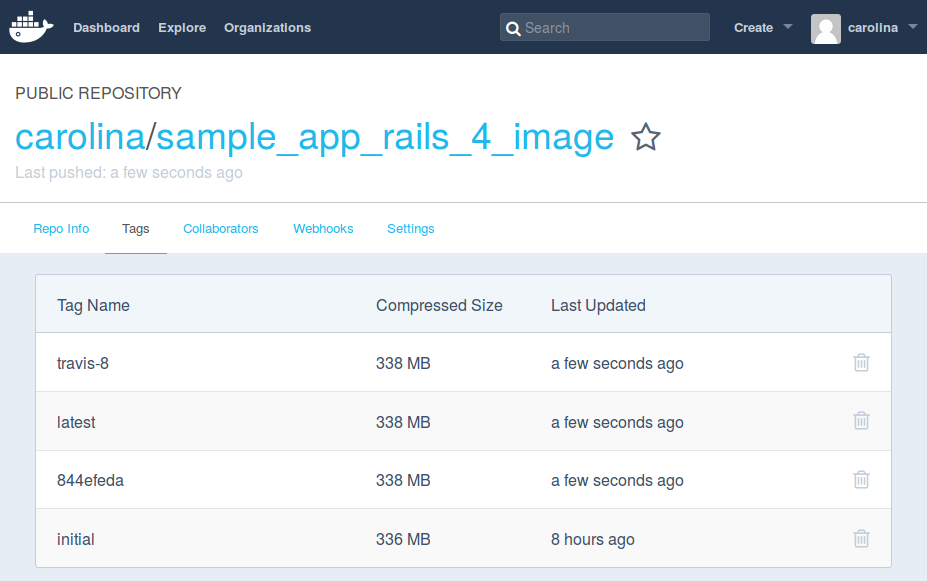
\includegraphics[width=0.8\textwidth]{images/figures/dockerhubimages.png}
\caption{Repositorio de \kode{sample\_app\_rails\_4\_image}.\label{fig:dockerhub_images}}
\end{figure}

\subsection{Vinculación con el repositorio remoto}

En primer lugar hay que ingresar en el sitio Travis CI con la cuenta de GitHub y añadir el repositorio con el que se trabaja actualmente:

\begin{figure}[H]
\image{images/figures/travis_github.png}
\caption{Vinculación de GitHub con Travis CI.\label{fig:travis_github}}
\end{figure}

\subsection{Configuración y establecimiento de precondiciones, condiciones y postcondiciones}

En segundo lugar se procede a instalar la nueva gema. Para ello se edita el fichero \kode{Gemfile}, incluyendo:

\begin{codelisting}
\label{code:addtravis}
\codecaption{Fichero \kode{Gemfile}}
%= lang:ruby
\begin{code}
.
group :development, :test do
  gem 'travis'
.
end
.
\end{code}
\end{codelisting} 

Luego se instala mediante:

%= lang:bash
\begin{code}
$ bundle install --without production
\end{code}

Una vez instalada, es necesario crear un nuevo fichero de configuración para la base de datos en Travis CI, que permitirá probar el correcto funcionamiento:
\begin{codelisting}
\label{code:travisdatabase}
\codecaption{Fichero \kode{config/database.yml.travis} }
%= lang:ruby
\begin{code}
test:
  adapter: postgresql
  database: travis_ci_test
  username: postgres
\end{code}
\end{codelisting}

Para configurar Travis CI se crea el fichero \kode{.travis.yml}. 

%= lang:bash
\begin{code}
$ touch .travis.yml
\end{code}

Tras ello, hay que establecer las variables de entorno correspondientes a las credenciales de DockerHub. Esto se especifica localmente mediante la ejecución de los siguientes comandos:

%= lang:bash
\begin{code}
$ travis env set DOCKER_USERNAME carolina
$ travis env set DOCKER_PASSWORD **************
\end{code}

También se agrega una variable de entorno que contenga los 8 primeros caracteres del \textit{hash} del \textit{git commit}, justo debajo de las anteriores.

En la sección \kode{after\_success} del fichero se inicia sesión en DockerHub y luego se construye la imagen. Al repositorio en DockerHub se subirán 3 copias comprimidas de la imagen. La primera etiquetada con el hash del \textit{commit} correspondiente, la segunda con el número de construcción en Travis CI y la tercera como la última versión, \textit{latest}. Además se le indica la base de datos de prueba para la ejecución de los tests y la versión de Ruby en uso.

El fichero definido queda de la siguiente forma:

\begin{codelisting}
\label{code:travis}
\codecaption{Fichero \kode{.travis.yml} }
%= lang:ruby
\begin{code}
env:
  global:
  - COMMIT=${TRAVIS_COMMIT::8}
language: ruby
rvm:
- 2.0.0-p648
bundler_args: --without production
addons:
  postgresql: '9.3'
services:
- docker
before_script:
- cp config/database.yml.travis config/database.yml
- psql -c 'create database travis_ci_test;' -U postgres
- RAILS_ENV=test bundle exec rake db:migrate --trace
script:
- bundle exec rspec
notifications:
  email:
    recipients:
    - c.santanamartel@gmail.com
    on_success: always
    on_failure: always
sudo: required
after_success:
- docker login -u $DOCKER_USERNAME -p $DOCKER_PASSWORD
- export REPO=$DOCKER_USERNAME/sample_app_rails_4_image
- docker build -f Dockerfile -t $REPO:$COMMIT .
- docker tag $REPO:$COMMIT $REPO:latest
- docker tag $REPO:$COMMIT $REPO:travis-$TRAVIS_BUILD_NUMBER
- docker push $REPO  
\end{code}
\end{codelisting}

Con la intención de compartir el repositorio GitHub con la comunidad, se crea una copia donde se borran manualmente las credenciales \kode{secure} para no exponerlas ya que, aunque esten encriptadas, si otro usuario hiciera uso del repositorio podría realizar nuevas subidas de imágenes en él, 
%= lang:bash
\begin{code}
$ cp .travis.yml .travis.yml.sample
\end{code}

Además se oculta el fichero \kode{.travis.yml} en GitHub y DockerHub:

\begin{codelisting}
\label{code:scriptdocker}
\codecaption{Añadido a los ficheros \kode{.gitignore} y \kode{.dockerignore}}
%= lang:bash
\begin{code}
.
.travis.yml
.
\end{code}
\end{codelisting}

\subsection{Resultado}

Finalmente, cuando se haga un nuevo \textit{commit} y subida al repositorio GitHub comenzará también la construcción en Travis CI. Tanto si se produce un fallo como si termina con éxito se ha configurado el envío de un correo electrónico para informarlo. Así, el caso de fallo se prueba comentando la línea que crea la base de datos de prueba \kode{travis\_ci\_test} y el de éxito con ella. De esta manera, los correos electrónicos recibidos son:

\begin{figure}[H]
\centering
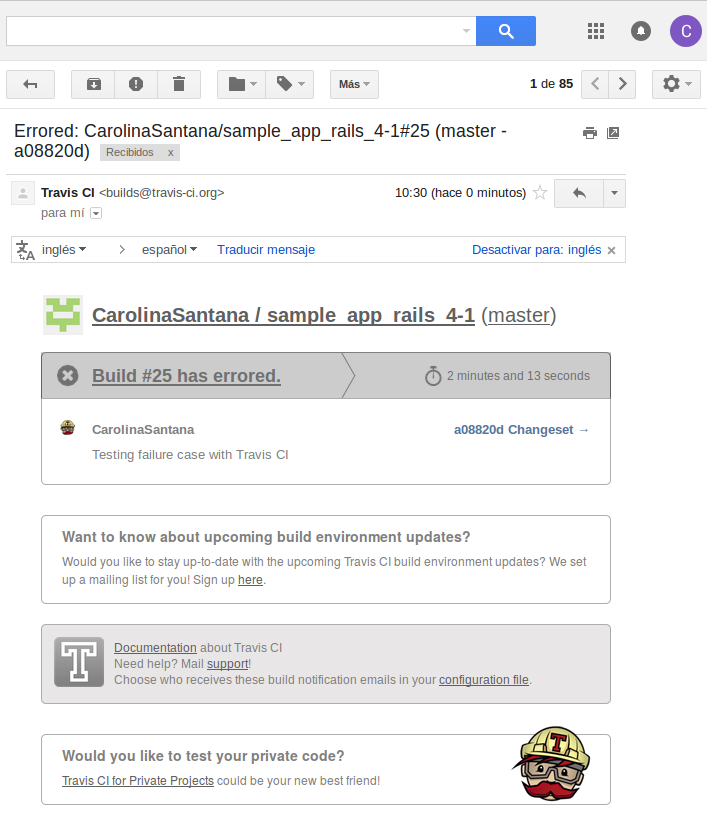
\includegraphics[width=0.7\textwidth]{images/figures/travisfailure.png}
\caption{Correo electrónico de Travis CI en caso de fallo.}
\end{figure}

\begin{figure}[H]
\centering
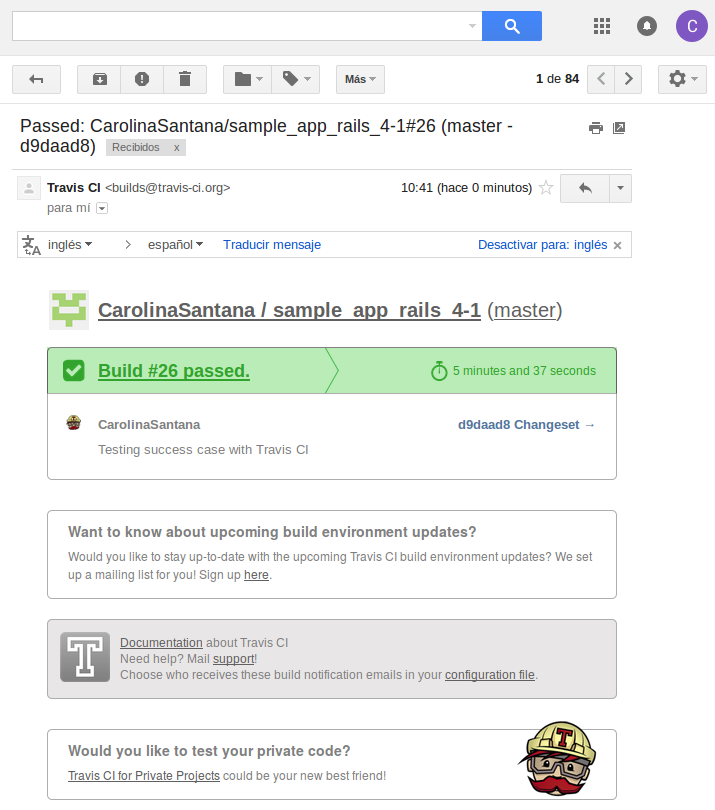
\includegraphics[width=0.7\textwidth]{images/figures/travissuccess.png}
\caption{Correo electrónico de Travis CI en caso de éxito.}
\end{figure}

Dirigiendo a Travis CI donde se comenta el fallo o el éxito:

\begin{figure}[H]
\centering
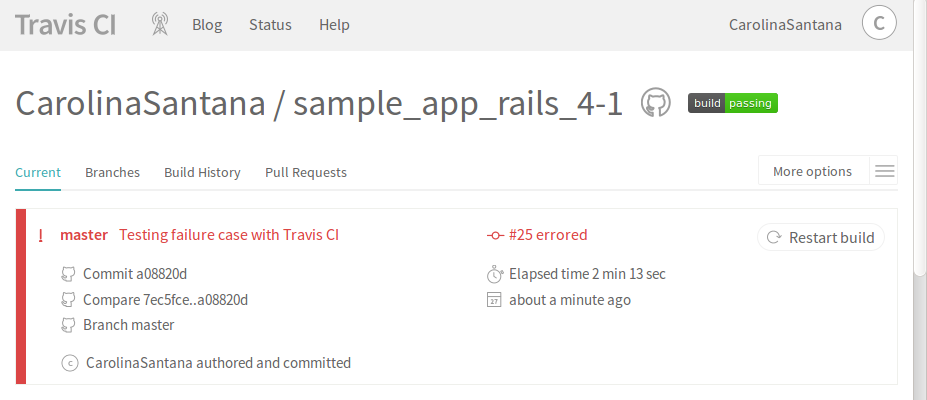
\includegraphics[width=0.8\textwidth]{images/figures/travisfailure2.png}
\caption{Caso de fallo en Travis CI.}
\end{figure}

\begin{figure}[H]
\centering
\image{images/figures/travisfailure3.png}
\caption{Motivo de fallo en Travis CI.}
\end{figure}

\begin{figure}[H]
\centering
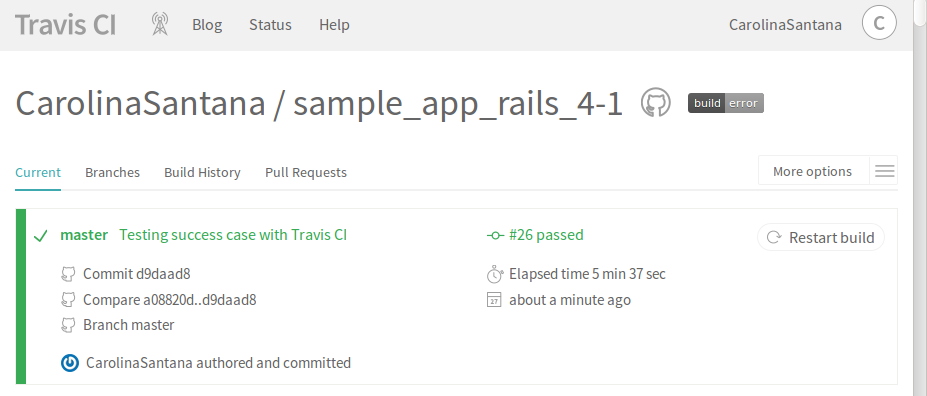
\includegraphics[width=0.8\textwidth]{images/figures/travissuccess2.png}
\caption{Caso de éxito en Travis CI.}
\end{figure}

Esta construcción terminará con la creación y subida de las tres imágenes comentadas en el planteamiento de esta iteración \ref{fig:dockerhub_images} en el repositorio de DockerHub.

\section{Iteración 4: Despliegue monomáquina con unidades de servicio usando Vagrant, VirtualBox y CoreOS}

En esta nueva iteración se quiere aplicar el uso del sistema operativo orientado a contenedores CoreOS. De esta manera se crearán unidades de servicio \kode{systemd} que se encargarán de realizar las tareas necesarias para la correcta aplicación y funcionamiento de los contenedores Docker en los que se divide la aplicación. Así, el nuevo planteamiento es el siguiente:

\begin{figure}[H] 
\centering
\image{images/figures/coreosdiagram.png}
\caption{Estructura del despliegue monomáquina con unidades de servicio CoreOS.\label{fig:coreosdiagram}}
\end{figure}

Se puede observar como en local existen dos herramientas de línea de comandos llamadas \kode{fleectl} y \kode{etcdctl} utilizadas internamente para comunicarse con los elementos del sistema CoreOS \kode{fleetd} y \kode{etcd}. Fleet se encarga de dotar a la máquina CoreOS los servicios que se desean implementar. Etcd permite almacenar las estructuras y datos pertinentes en la máquina CoreOS.

Para llevar a cabo esta iteración se utiliza el repositorio GitHub \kode{coreos/coreos-vagrant} que proporciona una plantilla \kode{Vagrantfile} para configurar el entorno de una máquina virtual CoreOS, usando el hipervisor software VirtualBox.

En este procedimiento hay tres archivos relevantes que se describirán a lo largo del proceso. De esta forma se utilizará la misma configuración para el fichero \kode{config.rb}, se creará un nuevo \kode{cloud-config} que será llamado \kode{user-data.sampleapp.virtualbox} y se modificará el fichero \kode{Vagranfile} en conveniencia.

\subsection{Preparación del repositorio local y remoto}

En primer lugar se realiza un \textit{fork} del repositorio \kode{coreos/coreos-vagrant} comentado seleccionando el botón con el mismo nombre y automáticamente se crea la copia del repositorio en la cuenta personal. Seguidamente se clona esta copia para trabajar localmente:

%= lang:bash
\begin{code}
$ git clone https://github.com/CarolinaSantana/coreos-vagrant.git 
\end{code}

Luego, se accede a la carpeta local que lo contiene y se prepara para comprobar su funcionamiento con los datos de usuario y la configuración de ejemplo. Esto se prueba ejecutando el \kode{Vagrantfile} y conectándose a la máquina virtual creada. En este caso se utiliza VirtualBox, lo que se conseguiría con \kode{vagrant up --provider=virtualbox} o \kode{vagrant up}, puesto que es el proveedor por defecto. 

%= lang:bash
\begin{code}
$ cd coreos-vagrant
$ cp user-data.sample user-data
$ cp config.rb.sample config.rb
$ vagrant up
$ vagrant ssh core-01
\end{code}

Comprobando que funciona correctamente:

\begin{figure}[H]
\image{images/figures/vagrantssh.png}
\caption{Conexión ssh a la máquina virtual \kode{core-01}.}
\end{figure}

Además puede visualizarse la máquina mediante VirtualBox:

\begin{figure}[H]
\centering
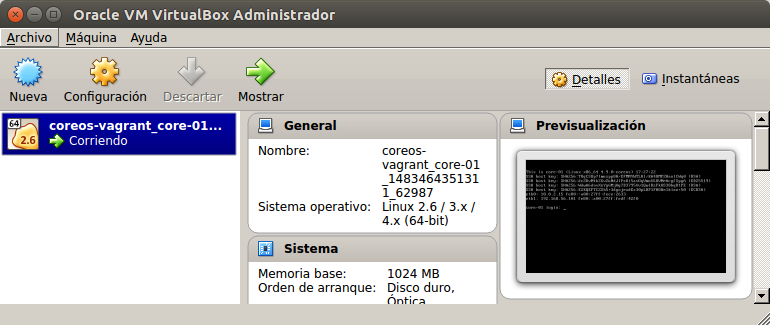
\includegraphics[width=0.8\textwidth]{images/figures/vboxcore01.png}
\caption{Máquina virtual \kode{core-01} desde VirtualBox.}
\end{figure}

\subsection{Interpretación de la cabecera del fichero user-data}

El fichero \kode{user-data} es el archivo de configuración \kode{cloud-config} que especifica el \kode{discovery token}, las variables de entorno y la lista de unidades de servicio que se deben iniciar de forma predeterminada. Vagrant copia el archivo \kode{cloud-config} en \kode{/var/lib/coreos-vagrant/vagrantfile-user-data}, dentro de la máquina virtual. De esta manera \kode{coreos-cloudinit} lee \kode{vagrantfile-user-data} en cada incio y lo utiliza para crear y reproducir el archivo de datos del usuario, \kode{user-data}, de la máquina.

Una vez que el entorno se ha comprobado y preparado para su uso se accede al fichero \kode{user-data} que contiene la lógica necesaria sobre los servicios \kode{etcd2}, \kode{fleet} y \kode{flannel}.

A efectos de CoreOS este fichero se denomina como \kode{cloud-config}. Los parámetros \kode{coreos.etcd}, \kode{coreos.fleet} y \kode{coreos.flannel} son traducidos a una unidad \kode{systemd} parcial actuando como un archivo de configuración \kode{etcd2}, \kode{fleet} y \kode{flannel}, respectivamente. 

Como el entorno de plataforma admite la función de plantilla de \kode{coreos-cloudinit}, es posible automatizar la configuración de \kode{etcd2} con los campos \kode{\$private\_ipv4} y \kode{\$public\_ipv4}. Al generar un \textit{discovery token} se establece el tamaño del clúster, ya que \kode{etcd2} lo utiliza para determinar si todos los miembros se han unido a él. Después de inicializarse, el clúster puede crecer o reducirse. Por su parte \kode{fleet} y \kode{flannel} usan variables de entorno en su configuración.

La siguiente sección de este fichero pertenece a las unidades de servicio, de las que ya se encuentran definidas \kode{etcd2.service}, \kode{fleet.service}, \kode{flanneld.service}, donde esta última especifica la red en CoreOS y \kode{docker-tcp.socket}, el cual permite que se pueda usar el servicio \kode{docker-service} dentro de cada máquina.

\begin{codelisting}
\label{code:cloud-config1}
\codecaption{Fichero \kode{user-data}}
%= lang:yaml
\begin{code}
#cloud-config
---
coreos:
  etcd2:
    advertise-client-urls: http://$public_ipv4:2379
    initial-advertise-peer-urls: http://$private_ipv4:2380
    listen-client-urls: http://0.0.0.0:2379,http://0.0.0.0:4001
    listen-peer-urls: http://$private_ipv4:2380,http://$private_ipv4:7001
    discovery: https://discovery.etcd.io/acd611cb07df434a400bbd7e36d793a0
  fleet:
    public-ip: "$public_ipv4"
  flannel:
    interface: "$public_ipv4"
  units:
  - name: etcd2.service
    command: start
  - name: fleet.service
    command: start
  - name: flanneld.service
    drop-ins:
    - name: 50-network-config.conf
      content: |
        [Service]
        ExecStartPre=/usr/bin/etcdctl set /coreos.com/network/config \
                     '{ "Network": "10.1.0.0/16" }'
    command: start
  - name: docker-tcp.socket
    command: start
    enable: true
    content: |
      [Unit]
      Description=Docker Socket for the API
      [Socket]
      ListenStream=2375
      Service=docker.service
      BindIPv6Only=both
      [Install]
      WantedBy=sockets.target
\end{code}
\end{codelisting}

Como este fichero pertenece a la configuración de ejemplo se realiza una copia del mismo para trabajar con el proveedor VirtualBox.

%= lang:bash
\begin{code}
$ cp user-data.sample user-data.sampleapp.virtualbox
\end{code}


\subsection{Interpretación del fichero config.rb}

El tercer fichero importante para este despliegue es \kode{config.rb}. Dicho fichero especifica el número de nodos CoreOS y proporciona una opción para generar automáticamente un \textit{discovery token}. Además permite la necesaria corrección del valor del parámetro perteneciente a la estrategia de reinicio de CoreOS, al tener que ser la entrada en el fichero \kode{user-data} de una manera distinta a como es tratado en CoreOS.

\begin{codelisting}
\label{code:cloud-config1}
\codecaption{Fichero \kode{config.rb}}
%= lang:ruby
\begin{code}
$num_instances=1
$new_discovery_url="https://discovery.etcd.io/new?size=#{$num_instances}"
if File.exists?('user-data') && ARGV[0].eql?('up')
  require 'open-uri'
  require 'yaml'
  token = open($new_discovery_url).read
  data = YAML.load(IO.readlines('user-data')[1..-1].join)
  if data.key? 'coreos' and data['coreos'].key? 'etcd'
    data['coreos']['etcd']['discovery'] = token
  end
  if data.key? 'coreos' and data['coreos'].key? 'etcd2'
    data['coreos']['etcd2']['discovery'] = token
  end
  # Fix for YAML.load() converting reboot-strategy from 'off' to `false`
  if data.key? 'coreos' and data['coreos'].key? 'update' 
    and data['coreos']['update'].key? 'reboot-strategy'
    if data['coreos']['update']['reboot-strategy'] == false
      data['coreos']['update']['reboot-strategy'] = 'off'
    end
  end
  yaml = YAML.dump(data)
  File.open('user-data', 'w') { |file| file.write("#cloud-config\n\n#{yaml}") }
end
\end{code}
\end{codelisting}

\subsection{Preparación del fichero Vagrantfile}

El fichero \kode{Vagrantfile} establece el tamaño del clúster CoreOS que ha de ser creado por Vagrant. En este caso una sola instancia. Además, señala el parámetro \textit{discovery token}, utilizado para la detección del tamaño del clúster, valor que se reemplaza automáticamente cuando se inicia el despliegue o levantamiento de una máquina, \kode{vagrant up}.

En este caso el fichero viene preparado para el uso de los proveedores VirtualBox y VMware. Al no utilizar el segundo se prescinde de sus configuraciones, así como se reagrupan las instrucciones pertinentes a VirtualBox.

También es importante recalcar que el fichero \kode{Vagrantfile} está preparado para hacer la copia del fichero \kode{user-data.sampleapp.virtualbox} a \kode{user-data}.

\begin{codelisting}
\label{code:cloud-config1}
\codecaption{Fichero \kode{Vagrantfile}}
%= lang:ruby
\begin{code}
# -*- mode: ruby -*-
# # vi: set ft=ruby :
require 'fileutils'
Vagrant.require_version ">= 1.6.0"
if (!ARGV.nil? && ARGV.join('').include?('provider=virtualbox')) || 
   (!ARGV.nil? && !ARGV.join('').include?('provider'))
  FileUtils.cp_r(File.join(File.dirname(__FILE__), \
  "user-data.sampleapp.virtualbox"), File.join(File.dirname(__FILE__), \
  "user-data"), :remove_destination => true)
end
CLOUD_CONFIG_PATH = File.join(File.dirname(__FILE__), "user-data")
CONFIG = File.join(File.dirname(__FILE__), "config.rb")
# Defaults for config options defined in CONFIG
$num_instances = 1
$instance_name_prefix = "core"
$update_channel = "alpha"
$image_version = "current"
$enable_serial_logging = false
$share_home = false
$vm_gui = false
$vm_memory = 1024
$vm_cpus = 1
$vb_cpuexecutioncap = 100
$shared_folders = {}
$forwarded_ports = {}
# Attempt to apply the deprecated environment variable NUM_INSTANCES to
# $num_instances while allowing config.rb to override it
if ENV["NUM_INSTANCES"].to_i > 0 && ENV["NUM_INSTANCES"]
  $num_instances = ENV["NUM_INSTANCES"].to_i
end
if File.exist?(CONFIG)
  require CONFIG
end
# Use old vb_xxx config variables when set
def vm_gui
  $vb_gui.nil? ? $vm_gui : $vb_gui
end
def vm_memory
  $vb_memory.nil? ? $vm_memory : $vb_memory
end
def vm_cpus
  $vb_cpus.nil? ? $vm_cpus : $vb_cpus
end
Vagrant.configure("2") do |config|
  # always use Vagrants insecure key
  config.ssh.insert_key = false
  # forward ssh agent to easily ssh into the different machines
  config.ssh.forward_agent = true
  config.vm.box = "coreos-%s" % $update_channel
  if $image_version != "current"
      config.vm.box_version = $image_version
  end
  config.vm.provider :virtualbox do |vb, override|
    override.vm.box_url = "https://storage.googleapis.com/%s.release.core-os.net/
    amd64-usr/%s/coreos_production_vagrant.json" %
    [$update_channel,$image_version]
    # On VirtualBox, we don't have guest additions or a functional vboxsf
    # in CoreOS, so tell Vagrant that so it can be smarter.
    vb.check_guest_additions = false
    vb.functional_vboxsf     = false
    #override.vm.provision "shell", path: "coreos-service-units-deploy.sh"
  end
  # plugin conflict
  if Vagrant.has_plugin?("vagrant-vbguest") then
    config.vbguest.auto_update = false
  end
  (1..$num_instances).each do |i|
    config.vm.define vm_name = "%s-%02d" % [$instance_name_prefix, i] do |config|
      config.vm.hostname = vm_name

      if $enable_serial_logging
        config.vm.provider :virtualbox do |vb, override|
          logdir = File.join(File.dirname(__FILE__), "log")
          FileUtils.mkdir_p(logdir)
          serialFile = File.join(logdir, "%s-serial.txt" % vm_name)
          FileUtils.touch(serialFile)
          vb.customize ["modifyvm", :id, "--uart1", "0x3F8", "4"]
          vb.customize ["modifyvm", :id, "--uartmode1", serialFile]
        end
      end
      if $expose_docker_tcp
        config.vm.provider :virtualbox do |vb, override|
          override.vm.network "forwarded_port", guest: 2375, host: 
          ($expose_docker_tcp + i - 1), host_ip: "127.0.0.1", auto_correct: true
        end
      end
      config.vm.provider :virtualbox do |vb, override|
        $forwarded_ports.each do |guest, host|
          override.vm.network "forwarded_port", guest: guest, host: host, 
          auto_correct: true
        end
        vb.gui = vm_gui
        vb.memory = vm_memory
        vb.cpus = vm_cpus
        vb.customize ["modifyvm", :id, "--cpuexecutioncap", 
                      "#{$vb_cpuexecutioncap}"]
        ip = "172.17.8.#{i+100}"
        override.vm.network :private_network, ip: ip
      end
      # Shared storage configuration
      config.vm.provider :virtualbox do |vb, override|
        # Uncomment below to enable NFS for sharing the host machine into the 
        # coreos-vagrant VM.
        #override.vm.synced_folder ".", "/home/core/share", id: "core", 
        #:nfs => true, :mount_options => ['nolock,vers=3,udp']
        $shared_folders.each_with_index do |(host_folder, guest_folder), index|
          override.vm.synced_folder host_folder.to_s, guest_folder.to_s, 
          id: "core-share%02d" % index, nfs: true, 
          mount_options: ['nolock,vers=3,udp']
        end
        if $share_home
          override.vm.synced_folder ENV['HOME'], ENV['HOME'], id: "home", 
          :nfs => true, :mount_options => ['nolock,vers=3,udp']
        end
      end
      # Copy of the cloud-config to the machine
      if File.exist?(CLOUD_CONFIG_PATH) && ARGV[0].eql?('up')
        config.vm.provider :virtualbox do |vb, override|
          override.vm.provision :file, :source => "#{CLOUD_CONFIG_PATH}", 
          :destination => "/tmp/vagrantfile-user-data"
          override.vm.provision :shell, :inline => "mv /tmp/vagrantfile-user-data \
          /var/lib/coreos-vagrant/", :privileged => true
        end
      end
    end
  end
end
\end{code}
\end{codelisting}

\subsection{Configuración y despliegue manual de las unidades de servicio systemd}

El primer paso consiste en permitir que exista almacenamiento NFS compartido entre la máquina local y la máquina virtual CoreOS, con la intención de poder pasar a esta última las unidades de servicio a implementar. Para ello es necesario descomentar la siguiente línea, dentro del fichero \kode{Vagrantfile}:

\begin{codelisting}
\label{code:vagrantfile2}
\codecaption{Fichero \kode{Vagrantfile}}
%= lang:ruby
\begin{code}
.
config.vm.synced_folder ".", "/home/core/share", id: "core", :nfs => true, \
:mount_options => ['nolock,vers=3,udp']
.
\end{code}
\end{codelisting}

También será necesario instalar el adaptador NFS en el sistema anfitrión y cargar los cambios. Esto creará, dentro de la máquina virtual, el directorio \kode{share}, compartido con el sistema anfitrión:

%= lang:bash
\begin{code}
$ sudo apt-get install nfs-kernel-server -y
$ vagrant reload --provision
\end{code}

\subsubsection{Unidad volume-public.service}

La primera unidad de servicio a crear será el volumen Docker compartido entre todos los contenedores. Para ello se crea, localmente, la ruta \kode{etc/sysctl/volume-public.service}. En este fichero se configura el servicio \kode{volume-public.service}. 

El contenido del mismo especifica que comenzará después de que lo haga el servicio Docker, el cual es requerido para el correcto funcionamiento. El servicio empezará directamente sin tiempo de espera. Una vez hecho se creará el volumen, añadiendo un enlace simbólico al mismo para todos los usuarios de la máquina. 

\begin{codelisting}
\label{code:volume-public.service}
\codecaption{Fichero \kode{etc/sysctl/volume-public.service}.}
%= lang:ruby
\begin{code}
[Unit] 
  Description= volume-public share between some-postgres, app-job, app-task and 
               some-nginx 
  After=docker.service
  Requires=docker.service
[Service] 
  TimeoutStartSec=0 
  ExecStart=/usr/bin/docker volume create --name volume-public
[Install] 
  WantedBy=multi-user.target
\end{code}
\end{codelisting}

\subsubsection{Unidad postgresql.service}

El siguiente paso consiste en agregar la unidades de servicio correspondiente a la base de datos de la aplicación. Para ello  se crea la ruta \kode{etc/sysctl/postgresql.service}. En este fichero se configura el servicio \kode{postgresql.service}.

El contenido del mismo especifica que comenzará después de que lo haga el servicio Docker y volume-public, requeridos para el correcto funcionamiento. El servicio empezará directamente sin tiempo de espera y se le indica el fichero donde ha de leer las variables de entorno necesarias. Si este servicio ya se ha ejecutado con anterioridad se procederá terminándolo y borrando el contenedor. Seguidamente, se comprobará, si ya existe la imagen del contenedor en la máquina, que sea la última versión disponible, de no ser así se obtendrá de nuevo. Llegado este punto la unidad de servicio comenzará creando el contenedor como se ha hecho hasta ahora, especificando la opción ha realizar si dicho contenedor quiere pararse. Además se añade un enlace simbólico al mismo para todos los usuarios de la máquina. 

\begin{codelisting}
\label{code:postgresql.service}
\codecaption{Fichero \kode{etc/sysctl/postgresql.service}.}
%= lang:ruby
\begin{code}
[Unit] 
  Description=PostgreSQL database 
  After=docker.service volume-public.service
  Requires=docker.service volume-public.service
[Service] 
  TimeoutStartSec=0
  EnvironmentFile=/home/core/share/etc/sysctl/postgres-credentials.env
  ExecStartPre=-/usr/bin/docker kill some-postgres 
  ExecStartPre=-/usr/bin/docker rm some-postgres 
  ExecStartPre=/usr/bin/docker pull postgres 
  ExecStart=/usr/bin/docker run --rm --name some-postgres \
  -e "POSTGRES_USER=${POSTGRES_USER}" \
  -e "POSTGRES_PASSWORD=${POSTGRES_PASSWORD}" \
  -v "volume-public:/var/lib/postgresql" -p "5432:5432" postgres 
  ExecStop=/usr/bin/docker stop some-postgres 
[Install] 
  WantedBy=multi-user.target
\end{code}
\end{codelisting}

El contenido del fichero que especifica las variables de entorno hace referencia a las credenciales de la base de datos. Esto es controlado por el servicio fleet para todos aquellos procesos en ejecución.

\begin{codelisting}
\label{code:credentials}
\codecaption{Contenido del fichero \kode{fleet\_machines.env}}
\begin{code}
POSTGRES_USER=postgres
POSTGRES_PASSWORD=postgres
\end{code}
\end{codelisting}

\subsubsection{Unidad app-job.service}

La siguiente unidad de servicio será el contenedor ejecutable de la aplicación que crea, migra y alimenta la base de datos. Para ello se crea la ruta \kode{etc/sysctl/app-job.service}. En este fichero se configura el servicio \kode{app-job.service}.

El contenido del mismo especifica que comenzará después de que lo haga el servicio Docker, volume-public y postgresql, requeridos para el correcto funcionamiento. El servicio empezará directamente sin tiempo de espera, indicándole el fichero donde ha de leer las variables de entorno necesarias. Si este servicio ya se ha ejecutado con anterioridad se procederá terminándolo y borrando el contenedor. Seguidamente, se comprobará, si ya existe la imagen del contenedor en la máquina, que sea la última versión disponible, de no ser así se obtendrá de nuevo. Llegado este punto la unidad de servicio comenzará creando el contenedor como se ha hecho hasta ahora, especificando la opción ha realizar si dicho contenedor quiere pararse. Además se añade un enlace simbólico al mismo para todos los usuarios de la máquina. 

\begin{codelisting}
\label{code:app-job.service}
\codecaption{Fichero \kode{etc/sysctl/app-job.service}.}
%= lang:ruby
\begin{code}
[Unit] 
  Description=executable app-job container that creates, migrates, seeds and 
              populates the database
  After=docker.service volume-public.service postgresql.service
  Requires=docker.service volume-public.service postgresql.service
[Service] 
  TimeoutStartSec=0 
  EnvironmentFile=/home/core/share/etc/sysctl/postgres-credentials.env
  ExecStartPre=-/usr/bin/docker kill app-job 
  ExecStartPre=-/usr/bin/docker rm app-job 
  ExecStartPre=/usr/bin/docker pull carolina/sample_app_rails_4_image:latest 
  ExecStart=/usr/bin/docker run --rm --name app-job \
  -v "volume-public:/usr/src/app/public" --entrypoint "/setup.sh" \
  -e "POSTGRES_USER=${POSTGRES_USER}" \
  -e "POSTGRES_PASSWORD=${POSTGRES_PASSWORD}" \
  -w "/usr/src/app" --link "some-postgres:db" \
  carolina/sample_app_rails_4_image:latest
[Install] 
  WantedBy=multi-user.target
\end{code}
\end{codelisting}

\subsubsection{Unidad app-task.service}

La siguiente unidad de servicio será el contenedor de la aplicación que ejecuta el servidor puma. Para ello se crea la ruta \kode{etc/sysctl/app-task.service}. En este fichero se configura el servicio \kode{app-task.service}.

El contenido del mismo especifica que comenzará después de que lo haga el servicio Docker, volume-public, postgresql y app-job, requeridos para el correcto funcionamiento. El servicio empezará directamente sin tiempo de espera, indicándole el fichero donde ha de leer las variables de entorno necesarias. Si este servicio ya se ha ejecutado con anterioridad se procederá terminándolo y borrando el contenedor. Seguidamente, se comprobará, si ya existe la imagen del contenedor en la máquina, que sea la última versión disponible, de no ser así se obtendrá de nuevo. Llegado este punto la unidad de servicio comenzará creando el contenedor como se ha hecho hasta ahora, especificando la opción ha realizar si dicho contenedor quiere pararse. Además se añade un enlace simbólico al mismo para todos los usuarios de la máquina. 

\begin{codelisting}
\label{code:app-task.service}
\codecaption{Fichero \kode{etc/sysctl/app-task.service}.}
%= lang:ruby
\begin{code}
[Unit] 
  Description=app-task container that runs the server puma
  After=docker.service volume-public.service postgresql.service app-job.service
  Requires=docker.service volume-public.service postgresql.service app-job.service
[Service] 
  TimeoutStartSec=0 
  EnvironmentFile=/home/core/share/etc/sysctl/postgres-credentials.env
  ExecStartPre=-/usr/bin/docker kill app-task 
  ExecStartPre=-/usr/bin/docker rm app-task
  ExecStartPre=/usr/bin/docker pull carolina/sample_app_rails_4_image:latest 
  ExecStart=/usr/bin/docker run --rm --name app-task \
  -e "POSTGRES_USER=${POSTGRES_USER}" \
  -e "POSTGRES_PASSWORD=${POSTGRES_PASSWORD}" \
  -w "/usr/src/app" -v "volume-public:/usr/src/app/public" \
  --link "some-postgres:db" carolina/sample_app_rails_4_image:latest \
  /bin/bash -c "cp config/database.yml.postgresql config/database.yml \
  && puma -p 9292"
  ExecStop=/usr/bin/docker stop app-task
[Install] 
  WantedBy=multi-user.target
\end{code}
\end{codelisting}

\subsubsection{Unidad nginx.service}

La siguiente unidad del servicio será el contenedor que ejecuta el servidor nginx. Para ello se crea la ruta \kode{etc/sysctl/nginx.service}. En este fichero se configura el servicio \kode{nginx.service}.

El contenido del mismo especifica que comenzará después de que lo haga el servicio Docker, volume-public, postgresql, app-job y app-task, requeridos para el correcto funcionamiento. El servicio empezará directamente sin tiempo de espera. Si este servicio ya se ha ejecutado con anterioridad se procederá terminándolo y borrando el contenedor. Seguidamente, se comprobará, si ya existe la imagen del contenedor en la máquina, que sea la última versión disponible, de no ser así se obtendrá de nuevo. Llegado este punto la unidad de servicio comenzará creando el contenedor como se ha hecho hasta ahora, teniendo en cuenta que ahora la redirección de puertos se ha establecido para trabajar el puerto 80 de la máquina CoreOS con el puerto 80 de la aplicación, especificando la opción ha realizar si dicho contenedor quiere pararse. Además se añade un enlace simbólico al mismo para todos los usuarios de la máquina. 

\begin{codelisting}
\label{code:nginx.service}
\codecaption{Fichero \kode{etc/sysctl/nginx.service}.}
%= lang:ruby
\begin{code}
[Unit] 
  Description=some-nginx container that runs a reverse proxy server and a 
              web server
  After=docker.service volume-public.service postgresql.service app-job.service 
        app-task.service
  Requires=docker.service volume-public.service postgresql.service 
           app-job.service app-task.service
[Service] 
  TimeoutStartSec=0 
  ExecStartPre=-/usr/bin/docker kill some-nginx 
  ExecStartPre=-/usr/bin/docker rm some-nginx
  ExecStartPre=/usr/bin/docker pull nginx 
  ExecStart=/usr/bin/docker run --rm --name some-nginx \
  -v "/home/core/share/etc/sysctl/nginx.conf:/etc/nginx/conf.d/default.conf" \
  -p "80:80" --link "app-task:app" -v "volume-public:/usr/src/app/public" nginx 
  ExecStop=/usr/bin/docker stop some-nginx
[Install] 
  WantedBy=multi-user.target
\end{code}
\end{codelisting}

\subsubsection{Despliegue manual}

Una vez que ya se han configurado y escrito las 5 unidades de servicio necesarias el siguiente paso es preparar su despliegue. Para el reconocimiento de las unidades éstas tienen que ubicarse bajo el servicio \kode{systemd}. Por ello el primer paso será la copia de las mismas al directorio \kode{/etc/systemd/system/}. El funcionamiento de las unidades pasa por dos estados. El primer estado es la habilitación del servicio, esto creará el enlace simbólico de la unidad para todos los usuarios. El segundo estado es el comienzo del mismo.

Dicho esto, se crea un script denominado \kode{coreos-service-units-deploy.sh}, con permisos \kode{chmod +x}, que se encargará de realizar la copia de las unidades bajo \kode{systemd} y que habilitará y comenzará los servicios.

\begin{codelisting}
\label{code:coreos-service-units-deploy}
\codecaption{Fichero \kode{coreos-service-units-deploy.sh}.}
%= lang:bash
\begin{code}
#!/bin/bash

sudo cp share/etc/sysctl/* /etc/systemd/system/
sudo systemctl enable volume-public.service
sudo systemctl enable postgresql.service
sudo systemctl enable app-job.service
sudo systemctl enable app-task.service
sudo systemctl enable nginx.service
sudo systemctl start volume-public.service
sudo systemctl start postgresql.service
sudo systemctl start app-job.service
sudo systemctl start app-task.service
sudo systemctl start nginx.service
\end{code}
\end{codelisting}

Con la intención de que este script se ejecute al iniciar la máquina CoreOS se añade al fichero \kode{Vagrantfile} una línea que indicará la ruta del mismo para hacer uso del fichero y provisionar la máquina con las directivas incluidas en él.

\begin{codelisting}
\label{code:vagrantfile3}
\codecaption{Fichero \kode{Vagrantfile}}
%= lang:ruby
\begin{code}
.
config.vm.provision "shell", path: "coreos-service-units-deploy.sh"
.
\end{code}
\end{codelisting}

Finalmente los pasos necesarios para iniciar la máquina serán la recarga de la misma con la opción de provisión, tanto por el hecho de que la máquina pueda encontrarse ya iniciada y por si se han hecho cambios en los ficheros que influyen en la construcción de los servicios internos a llevar a cabo. Además, habrá que acceder a dicha máquina. 

%= lang:bash
\begin{code}
$ vagrant reload --provision
$ vagrant ssh core-01
\end{code}

Si se inicia el despliegue manual se comprueba el correcto funcionamiento de la aplicación, donde todos los servicios estarán en estado activo o cargado:

\begin{figure}[H]
\centering
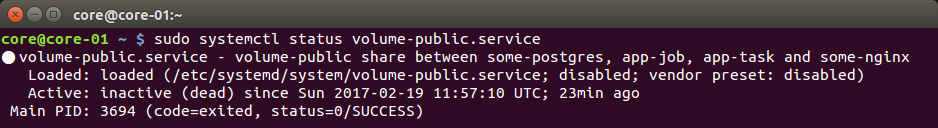
\includegraphics[width=1\textwidth]{images/figures/volume-public.service.png}
\caption{Estado de la unidad \kode{volume-public.service}.}
\end{figure}

\begin{figure}[H]
\centering
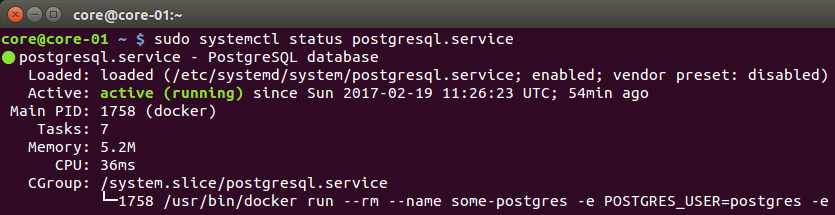
\includegraphics[width=0.8\textwidth]{images/figures/postgresql.service.png}
\caption{Estado de la unidad \kode{postgresql.service}..}
\end{figure}

\begin{figure}[H]
\centering
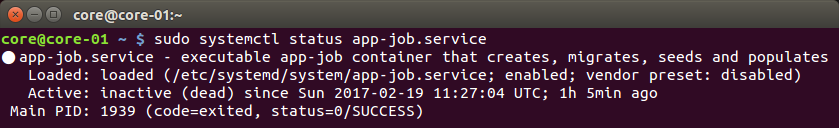
\includegraphics[width=0.8\textwidth]{images/figures/app-job.service.png}
\caption{Estado de la unidad \kode{app-job.service}.}
\end{figure}

\begin{figure}[H]
\centering
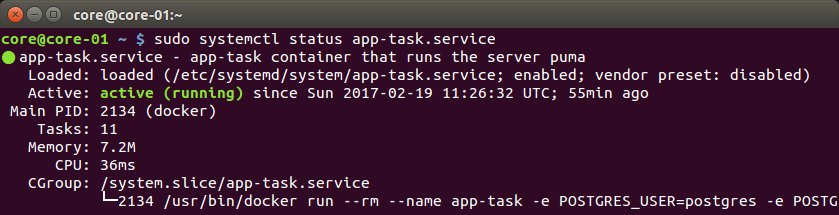
\includegraphics[width=0.8\textwidth]{images/figures/app-task.service.png}
\caption{Estado de la unidad \kode{app-task.service}.}
\end{figure}

\begin{figure}[H]
\centering
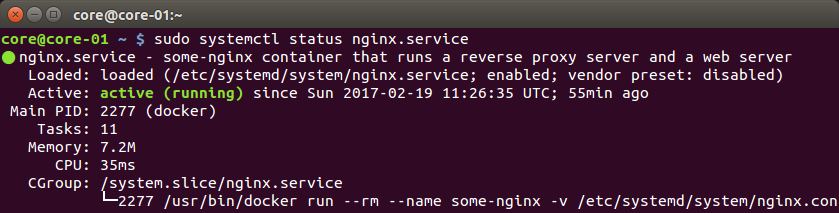
\includegraphics[width=0.8\textwidth]{images/figures/nginx.service.png}
\caption{Estado de la unidad \kode{nginx.service}.}
\end{figure}

Por último se accede a la aplicación en modo consola desde la máquina CoreOS y en modo gráfico desde el sistema anfitrión:

\begin{figure}[H]
\centering
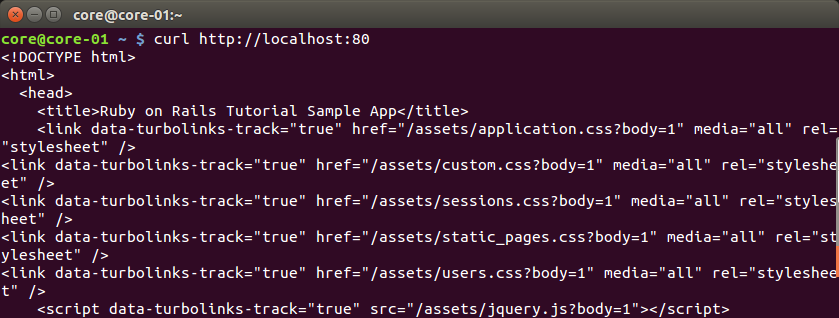
\includegraphics[width=0.8\textwidth]{images/figures/coreosmanualcurl.png}
\caption{Acceso a la aplicación desde la máquina CoreOS.}
\end{figure}

\begin{figure}[H]
\centering
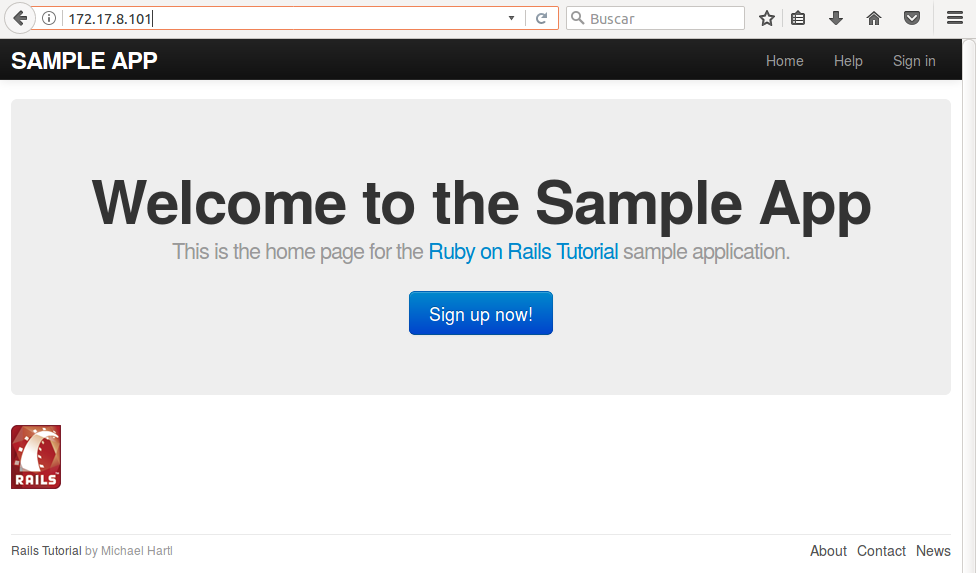
\includegraphics[width=0.7\textwidth]{images/figures/coreosmanualhost.png}
\caption{Acceso a la aplicación desde el sistema anfitrión.}
\end{figure}

\subsection{Configuración y despliegue automático de las unidades de servicio systemd}

El despliegue ideal de la aplicación a través de las unidades de servicio que la componen sería de manera automática. Esto se implementa en CoreOS a partir del fichero denominado \kode{cloud-config} que se corresponde con \kode{user-data}. Este fichero especifica el orden de las unidades a desplegar y las acciones de habilitación y comienzo de los servicios a los que hacen referencia.

Esta vez no se usará el almacenamiento NFS compartido así que el fichero con las variables de entorno también es descrito, índicandole la nueva ruta en la que se encuentra, sus permisos y contenido encodificado en base64. Lo mismo se realiza para el fichero que contiene la configuracińo nginx, sin encodificar.

Así, la confección de este fichero, que recibirá el nombre de \kode{user-data.sampleapp.sample.virtualbox}, queda de la siguiente manera:

\begin{codelisting}
\label{code:vagrantfile2}
\codecaption{Fichero \kode{user-data.sampleapp.virtualbox}}
%= lang:yaml
\begin{code}
#cloud-config
---
write_files:
  - path: "/etc/postgres-credentials.env"
    permissions: "0644"
    content: |
      POSTGRES_USER=postgres
      POSTGRES_PASSWORD=postgres
  - path: "/etc/nginx.conf"
    permissions: "0644"
    content: |
      server {
        listen 80;
        root /usr/src/app/public;
        location / {
          proxy_set_header X-Forwarded-For $proxy_add_x_forwarded_for;
          proxy_set_header Host $http_host;
          proxy_redirect off;
          try_files $uri /page_cache/$uri /page_cache/$uri.html @app;
        }
        location @app{
          proxy_pass http://app:9292;
          break;
        }
      }
coreos:
  etcd2:
    advertise-client-urls: http://$public_ipv4:2379
    initial-advertise-peer-urls: http://$private_ipv4:2380
    listen-client-urls: http://0.0.0.0:2379,http://0.0.0.0:4001
    listen-peer-urls: http://$private_ipv4:2380,http://$private_ipv4:7001
    discovery: https://discovery.etcd.io/e26b5e212eaa7df4a003cee8bac6ed16
  fleet:
    public-ip: "$public_ipv4"
  flannel:
    interface: "$public_ipv4"
  units:
  - name: etcd2.service
    command: start
  - name: fleet.service
    command: start
  - name: flanneld.service
    drop-ins:
    - name: 50-network-config.conf
      content: |
        [Service]
        ExecStartPre=/usr/bin/etcdctl set /coreos.com/network/config 
                     '{ "Network": "10.1.0.0/16" }'
    command: start
  - name: docker-tcp.socket
    command: start
    enable: true
    content: |
      [Unit]
      Description=Docker Socket for the API
      [Socket]
      ListenStream=2375
      Service=docker.service
      BindIPv6Only=both
      [Install]
      WantedBy=sockets.target
  - name: volume-public.service
    command: start
    enable: true
    content: |
      [Unit] 
      Description= volume-public share between some-postgres, app-job, app-task
                   and some-nginx 
      After=docker.service
      Requires=docker.service
      [Service] 
      TimeoutStartSec=0 
      ExecStart=/usr/bin/docker volume create --name volume-public
      [Install] 
      WantedBy=multi-user.target
  - name: postgresql.service
    command: start
    enable: true
    content: |
      [Unit] 
      Description=PostgreSQL database 
      After=docker.service volume-public.service
      Requires=docker.service volume-public.service
      [Service] 
      TimeoutStartSec=0
      EnvironmentFile=/etc/postgres-credentials.env
      ExecStartPre=-/usr/bin/docker kill some-postgres 
      ExecStartPre=-/usr/bin/docker rm some-postgres 
      ExecStartPre=/usr/bin/docker pull postgres 
      ExecStart=/usr/bin/docker run --rm --name some-postgres \
      -e "POSTGRES_USER=${POSTGRES_USER}" \
      -e "POSTGRES_PASSWORD=${POSTGRES_PASSWORD}" \
      -v "volume-public:/var/lib/postgresql" -p "5432:5432" postgres 
      ExecStop=/usr/bin/docker stop some-postgres
      [Install] 
      WantedBy=multi-user.target
  - name: app-job.service
    command: start
    enable: true
    content: |
      [Unit] 
      Description=executable app-job container that creates, migrates, seeds
                  and populates the database
      After=docker.service volume-public.service postgresql.service
      Requires=docker.service volume-public.service postgresql.service
      [Service] 
      TimeoutStartSec=0 
      EnvironmentFile=/etc/postgres-credentials.env
      ExecStartPre=-/usr/bin/docker kill app-job 
      ExecStartPre=-/usr/bin/docker rm app-job 
      ExecStartPre=/usr/bin/docker pull carolina/sample_app_rails_4_image:latest 
      ExecStart=/usr/bin/docker run --rm --name app-job \
                -v "volume-public:/usr/src/app/public" --entrypoint "/setup.sh" \
      -e "POSTGRES_USER=${POSTGRES_USER}" \
      -e "POSTGRES_PASSWORD=${POSTGRES_PASSWORD}" \
      -w "/usr/src/app" --link "some-postgres:db" \
      carolina/sample_app_rails_4_image:latest
      [Install] 
      WantedBy=multi-user.target
  - name: app-task.service
    command: start
    enable: true
    content: |
      [Unit] 
      Description=app-task container that runs the server puma
      After=docker.service volume-public.service postgresql.service 
            app-job.service
      Requires=docker.service volume-public.service postgresql.service 
               app-job.service
      [Service] 
      TimeoutStartSec=0 
      EnvironmentFile=/etc/postgres-credentials.env
      ExecStartPre=-/usr/bin/docker kill app-task 
      ExecStartPre=-/usr/bin/docker rm app-task
      ExecStartPre=/usr/bin/docker pull carolina/sample_app_rails_4_image:latest 
      ExecStart=/usr/bin/docker run --rm --name app-task \
      -e "POSTGRES_USER=${POSTGRES_USER}" \
      -e "POSTGRES_PASSWORD=${POSTGRES_PASSWORD}" \
      -w "/usr/src/app" -v "volume-public:/usr/src/app/public" \
      --link "some-postgres:db" carolina/sample_app_rails_4_image:latest \
      /bin/bash -c "cp config/database.yml.postgresql \
      config/database.yml && puma -p 9292"
      ExecStop=/usr/bin/docker stop app-task
      [Install] 
      WantedBy=multi-user.target
  - name: nginx.service
    command: start
    enable: true
    content: |
      [Unit] 
      Description=some-nginx container that runs a reverse proxy server and 
                  a web server
      After=docker.service volume-public.service postgresql.service 
            app-job.service app-task.service
      Requires=docker.service volume-public.service postgresql.service 
               app-job.service app-task.service
      [Service] 
      TimeoutStartSec=0 
      ExecStartPre=-/usr/bin/docker kill some-nginx 
      ExecStartPre=-/usr/bin/docker rm some-nginx
      ExecStartPre=/usr/bin/docker pull nginx 
      ExecStart=/usr/bin/docker run --rm --name some-nginx \
      -v "/etc/nginx.conf:/etc/nginx/conf.d/default.conf" \
      -p "80:80" --link "app-task:app" \
      -v "volume-public:/usr/src/app/public" nginx 
      ExecStop=/usr/bin/docker stop some-nginx
      [Install] 
      WantedBy=multi-user.target
  \end{code}
\end{codelisting}

Como ya no es necesario el almacenamiento NFS compartido ya no hay que realizar la copia de los ficheros de las unidades del entorno local a la máquina CoreOS. Por lo tanto ya no es necesaria la línea de provisión del script en el fichero \kode{Vagranfile}. Además, puede volver a comentarse la línea que habilitaba este tipo de almacenamiento.

El fichero es validado con la utilidad \textit{Config Validator}\footnotettt{Config Validator}{https://coreos.com/validate}. 

Si se inicia el despliegue se comprueba el correcto funcionamiento de la aplicación, nuevamente.

%= lang:bash
\begin{code}
$ vagrant up
$ vagrant ssh core-01
\end{code}

\subsection{Resultado}

Tanto si se decide realizar el despliegue manual o automático con unidades usando CoreOS se obtiene el correcto funcionamiento de la aplicación a través de cada servicio independiente.

El resultado en ambos casos ha sido positivo:

\begin{figure}[H]
\centering
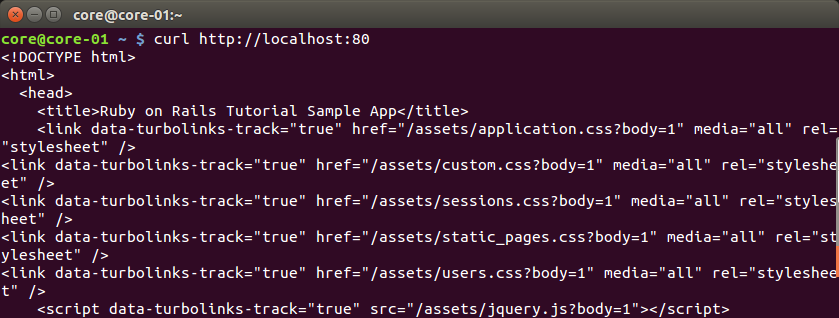
\includegraphics[width=0.7\textwidth]{images/figures/coreosmanualcurl.png}
\caption{Despliegue manual y automático. Acceso desde la máquina CoreOS.}
\end{figure}

\begin{figure}[H]
\centering
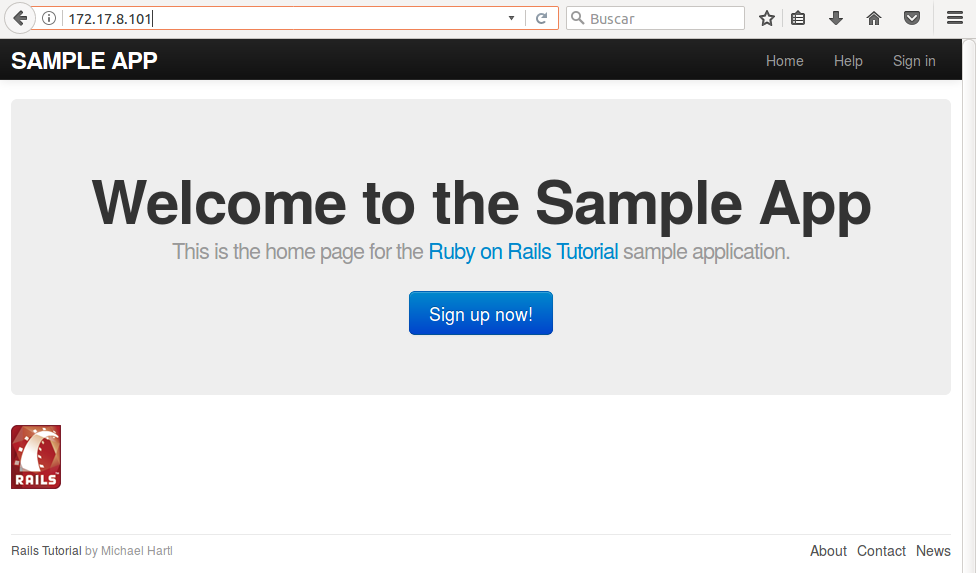
\includegraphics[width=0.7\textwidth]{images/figures/coreosmanualhost.png}
\caption{Despliegue manual y automático. Acceso desde el sistema anfitrión.}
\end{figure}

\section{Iteración 5: Despliegue en la nube pública de Amazon Web Services}

En esta iteración se pretende desplegar la infraestructura en la nube pública de AWS. Para ello se trabajará el mismo fichero \kode{config.rb}, el nuevo \kode{user-data.sampleapp.aws} personalizado, así como se harán una serie de variaciones en el fichero \kode{Vagrantfile}, introduciendo las instrucciones necesarias para el tratamiento e integración del proveedor AWS.

Así, la distribución de las unidades de servicio y, por tanto, de los contenedores quedará de la siguiente forma:

\begin{figure}[H]
\centering
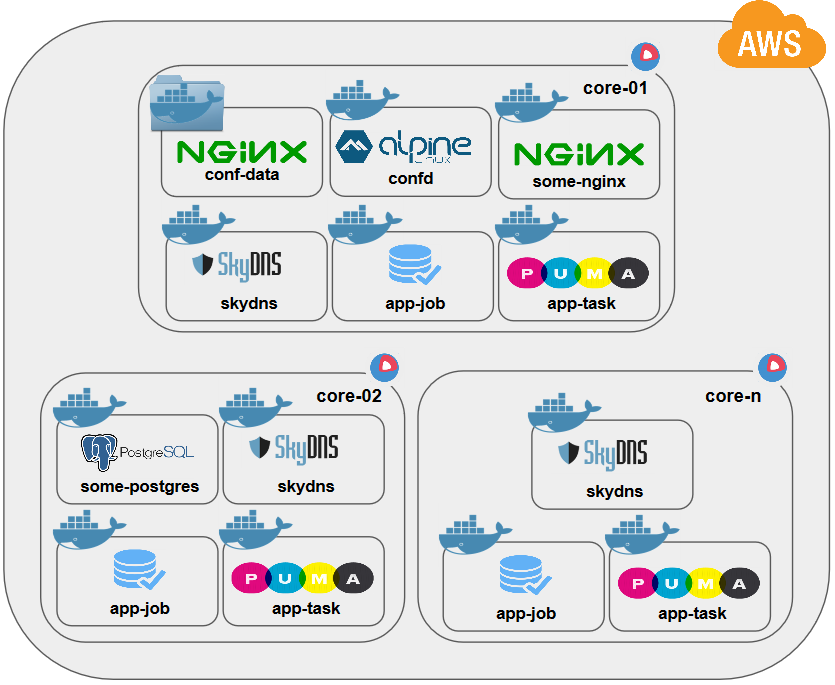
\includegraphics[width=0.75\textwidth]{images/figures/aws-1-iteration.png}
\caption{Distribución de la infraestructura a desplegar en la nube pública de Amazon Web Services.}
\end{figure}

En ella puede distinguirse que el proxy, presente en el contenedor \kode{some-nginx}, que redirige al servidor web de la aplicación se encuentra en la máquina \kode{core-01}. Nginx será el servicio al cual los clientes y usuarios finales realizan las peticiones para acceder a la aplicación. No obstante, no solo se va a tener un servidor de la aplicación, si no que éste puede estar replicado desde en una a todas las instancias de la infraestructura y el servicio nginx deberá balancear la carga entre ellos. Para poder controlar los servidores web que se registran y/o dejan de estar en el sistema se implementará un nuevo contenenedor, \kode{confd}, y un nuevo volumen Docker, \kode{conf-data}. A su vez, el contenedor \kode{some-postgres} para la base de datos se ubicará en la máquina \kode{core-02}. A él tiene que acceder tanto el contenedor \kode{app-job}, que la crea, migra y alimenta, como el contenedor \kode{app-task} que se dirige al mismo para obtener y escribir la información solicitada y añadida en la aplicación web. Ello se consigue con la implementación del contenedor \kode{skydns} que servirá como servidor DNS a estos dos contenedores, trabajando con las claves y valores de etc2.

La relación entre los contenedores, independientemente de su ubicación y replicación en otras instancias, en la manera en la que se ha comentado, puede apreciarse con mayor detalle en la siguiente figura:

\begin{figure}[H]
\centering
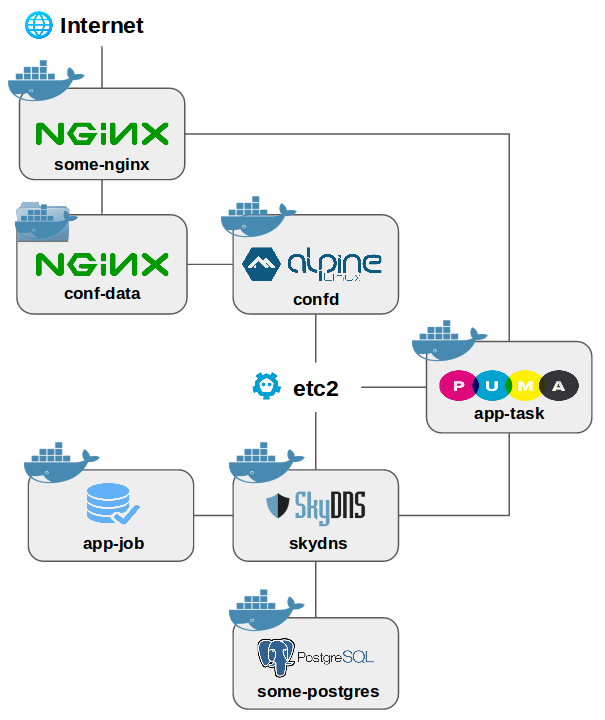
\includegraphics[width=0.6\textwidth]{images/figures/aws-2-iteration.png}
\caption{Relación entre los contenedores de la Infraestructura.}
\end{figure}

Cuando la infraestructura se despliega, el contenedor \kode{some-postgres}, donde será alojada la base de datos, se registra en el servidor DNS, \kode{skydns}. Éste utiliza etc2 para almacenar las claves y valores. De esta manera, \kode{some-postgres} puede ser descubierto por los contenedores \kode{app-job}, uno de los cuales, el primero, creará, migrará y alimentará la base de datos. Cuando arrancan los contenedores \kode{app-task}, servidores web de la aplicación, se registran en etc2. El contenedor \kode{confd} vigila estos cambios cada 5 segundos para actualizar la configuración de \kode{some-nginx} y pueda resolver hacia ellos. Puesto que se comparte un fichero entre dos contenedores se utiliza el volumen \kode{conf-data}. Así, cuando un cliente realiza una petición a través de Internet a \kode{some-nginx}, éste puede redirigirle a uno de los servidores \kode{app-task}, el cuál consultará \kode{skydns} para poder obtener y escribir información en la base de datos. La política para redireccionar a los servidores web será \textit{Round Robin}, del primero al último.

Al ya no estar los contenedores en la misma instancia, compartir el volumen Docker \kode{volume-public} de la manera en la que se ha ido haciendo no es posible. Como no es el propósito directo del presente trabajo su implementación se descontinúa y su tratamiento será incorporado en la sección de Trabajos Futuros \ref{trabajosfuturos}.

El servicio quedará disponible mediante el despliegue de la infraestructura desde Vagrant, estableciendo antes las variables de entorno correspondientes al proveedor. El acceso correcto al servicio puede ser probado desde la máquina \kode{core-01}, que contiene el proxy:

%= lang:bash
\begin{code}
$ . ~/.aws-credentials/aws-credentials
$ vagrant up --provider=aws
$ vagrant ssh core-01
# curl http://localhost:80
\end{code}

\begin{figure}[H]
\centering
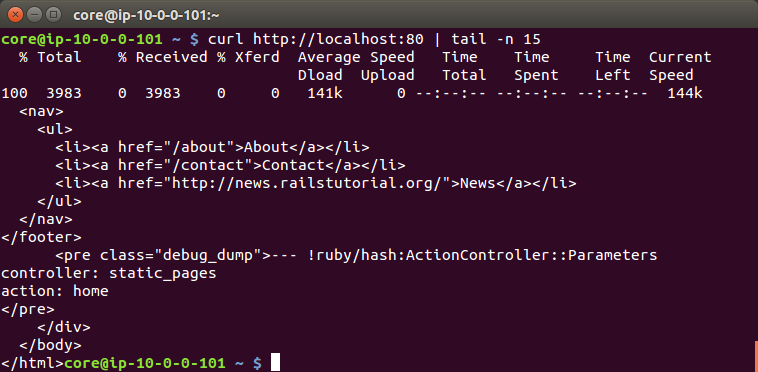
\includegraphics[width=0.7\textwidth]{images/figures/curl-confd.png}
\caption{Respuesta al servicio por comandos en \kode{core-01}.}
\end{figure}

\subsection{Obtención de la cuenta AWS}

Para la realización de esta iteración es necesario crear una cuenta en Amazon Web Services. En el caso presente se utilizará una cuenta que posee una capa gratuita, con una duración de un año, que se usa en conjunto con un crédito de \$50 dólares, proporcionado por dicha entidad. Este crédito ha sido facilitado al pertenecer al programa \textit{AWS Educate}\footnotettt{AWS Educate}{https://aws.amazon.com/es/grants/}. Se trata de una iniciativa de Amazon a nivel mundial que proporciona a los estudiantes y personal docente los recursos necesarios para acelerar el aprendizaje relacionado con la nube, así como para ayudar a formar a futuros empresarios e investigadores.

Los servicios de AWS se localizan en múltiples ubicaciones por todo el mundo. Así, tienen diferentes regiones y, en cada una de ellas, distintas zonas de disponibilidad. En este proyecto se escogerá la región US East y zona N. Virginia.

Se hace uso del servicio AWS Identity and Access Management (IAM) con la intención de controlar de forma segura el acceso a servicios y recursos por parte del usuario. Así, con el objetivo de tener un usuario para solamente actividades de desarrollo, el primer paso será la creación del grupo \textit{deployers} con permiso para manejar las instancias EC2. Luego, se crea el usuario \textit{deployer} con tipo de acceso \textit{AWS Management Console access}. Al mismo se le facilita una contraseña y se le indica que pertenece al grupo recién creado.

A partir de ahora se trabajará en la cuenta AWS bajo este usuario.

\subsection{Creación de la red y subred virtual}

El servicio Virtual Private Cloud (VPC) permite controlar todos los aspectos del entorno de red virtual. Será usado con la intención de hacer la selección del rango de direcciones IP que se les dará a las máquinas virtuales, así como para crear una subred acorde.

En primer lugar se crea una VPC llamada \textit{vpc-sampleapp} con el rango de direcciones IPv4 como bloque de enrutamiento entre dominios sin clases (CIDR) 10.0.0.0/16:

\begin{figure}[H]
\centering
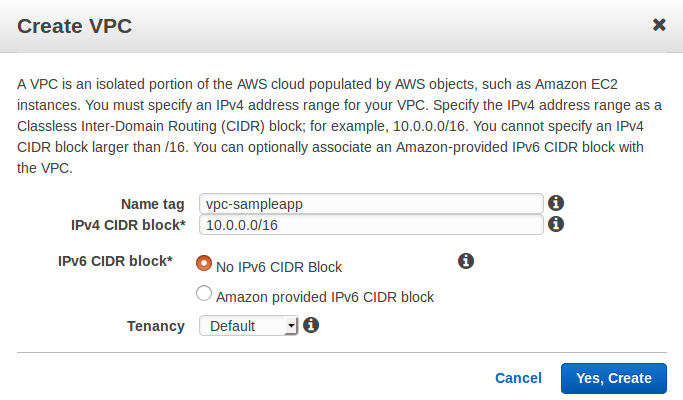
\includegraphics[width=0.7\textwidth]{images/figures/vpc-sampleapp.png}
\caption{Creación de la VPC vpc-sampleapp.}
\end{figure}

En segundo lugar se crea una subred llamada \textit{subnet-sampleapp} perteneciente a la anterior VPC y con el rango de direcciones IPv4 como bloque de enrutamiento entre dominios sin clases (CIDR) 10.0.0.0/24:

\begin{figure}[H]
\centering
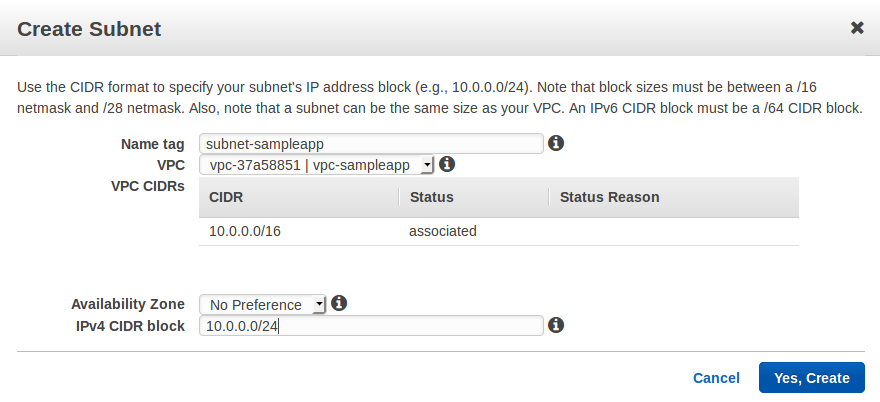
\includegraphics[width=0.8\textwidth]{images/figures/subnet-sampleapp.png}
\caption{Creación de la subred subnet-sampleapp.}
\end{figure}

\subsection{Creación del par de claves y del grupo de seguridad}

Lo siguiente es preparar una pareja de claves \textit{key pair} para poder entrar por SSH en la instancia que se lance para su ejecución. Para ello es necesario crear un \textit{Security Group} que defina los puertos de entrada a través de los que la instancia podrá recibir peticiones.

Lo primero se realiza accediendo al servicio Amazon Elastic Cloud Computing (Amazon EC2) y navegando hasta \textit{Network \& Security, Key Pairs}. Aquí, se crea una nueva pareja de claves con el nombre \kode{keypair.pem}, la cual se guarda en un directorio oculto que se crea con el nombre de \kode{\textasciitilde{}/.aws-credentials}, facilitándole los permisos de lectura y escritura al propietario:

%= lang:bash
\begin{code}
$ mkdir ~/.aws-credentials
$ mv /home/carolina/Descargas/keypair.pem ~/.aws-credentials/
$ chmod 0600 ~/.aws-credentials/keypair.pem
\end{code}

Ahora se navega hasta \textit{Network \& Security, Security Groups} y se crea el grupo de seguridad \textit{deploying-security-group} con las reglas TCP entrantes que permitan dejar pasar a la instancia las peticiones que llegan para conexiones a los puertos asignados a los protocolos SSH (22) y HTTP (80). También se añaden las reglas TCP a los puertos que utiliza CoreOS en sus comunicaciones con los clientes, siendo 2379, 2380, 4001, 7001. Con la intención de que, en un momento dado, las distintas máquinas virtuales que se creen formando un clúster CoreOS tengan conectividad con los contenedores de otras máquinas virtuales miembro se habilita el puerto 8285 mediante una regla UDP. Finalmente, se añaden las reglas TCP sobre los puertos que afectan a la aplicación, 9292 para el servidor puma y 5432 para el servidor PostgreSQL.

\subsection{Configuración del fichero user-data}

Para poder llevar a cabo esta parte se necesita una nueva configuración \kode{cloud-config}. Este nuevo \kode{user-data} recibirá el nombre de \kode{user-data.sampleapp.aws}. Tendrá, únicamente, dos diferencias respecto al anterior, por ello se copia:

%= lang:bash
\begin{code}
$ cp user-data.sampleapp.virtualbox user-data.sampleapp.aws
\end{code}

La primera de las diferencias será especificar al servicio flannel que ha de usar el rango de direcciones IPv4 privadas, pues los contenedores internos a la máquina usarán una red privada. El segundo cambio detalla que la red privada a usar será la 172.17.0.0/16 y el protocolo UDP.

\begin{codelisting}
\label{code:vagrantfile2}
\codecaption{Detalles a cambiar en el fichero \kode{user-data.sampleapp.aws}}
%= lang:yaml
\begin{code}
.
coreos:
  .
  flannel:
    interface: "$private_ipv4"
  units:
  .
  - name: flanneld.service
    drop-ins:
    - name: 50-network-config.conf
      content: |
        [Service]
        ExecStartPre=/usr/bin/etcdctl set /coreos.com/network/config 
               '{ "Network": "172.17.0.0/16", "Backend": { "Type": "udp" } }'
.
\end{code}
\end{codelisting}

\subsection{Configuración del fichero Vagrantfile}

En primer lugar se instala el plugin necesario para poder utilizar AWS como proveedor:

%= lang:bash
\begin{code}
$ vagrant plugin install vagrant-aws
\end{code}

Al fichero \kode{Vagrantfile} es necesario añadirle la comprobación de que se encuentre instalado en el sistema anfitrión el plugin \kode{vagrant-aws}, necesario para trabajar con ambas tecnologías.

Para poder iniciar sesión en la cuenta AWS como usuario \textit{deployer} se agregará un fichero local en el que especificar estos datos sensibles, con la intención de ser tratados como variables de entorno. Para ello se crea el fichero \kode{\textasciitilde{}/.aws-credentials/aws-credentials} con permiso de ejecución \textit{chmod +x} con el contenido:

\begin{codelisting}
\label{code:vagrantfile2}
\codecaption{Fichero \kode{\textasciitilde{}/.aws-credentials/aws-credentials}}
%= lang:bash
\begin{code}
export AWS_KEY='XXXXXXXXXXXXXXXXXXX'
export AWS_SECRET='XXXXXXXXXXXXXXXXXXXXXXXXXXX'
export AWS_KEYNAME='keypair'
export AWS_KEYPATH='~/.aws-credentials/keypair.pem'
\end{code}
\end{codelisting}

Así, en el propio \kode{Vagrantfile} se especificará que las variables de entorno \kode{ENV['AWS\_KEY']}, \kode{ENV['AWS\_SECRET']} y \kode{ENV['AWS\_KEYNAME']} deben estar establecidas para poder continuar. Para ello se ejecuta en el directorio actual:

%= lang:bash
\begin{code}
$ . ~/.aws-credentials/aws-credentials
\end{code}

Luego, como en el caso anterior, se prepara la copia del fichero \kode{cloud-config} de \kode{user-data.sampleapp.aws} a \kode{user-data}.

Todas las opciones necesarias para el despliegue desde Vagrant con este proveedor vienen a determinar la configuración de la instancia o instancias a lanzar. Las características que interesan definir son las siguientes:
\begin{itemize}
\item \textit{access\_key\_id}: Primera clave, perteneciente al identificador del usuario.
\item \textit{secret\_access\_key}: Segunda clave, perteneciente a la contraseña secreta.
\item \textit{keypair\_name}: Nombre del archivo que contiene el par de claves.
\item \textit{aws\_region}: Región.
\item \textit{aws\_availability\_zone}: Zona de disponibilidad.
\item \textit{aws\_subnet\_id}: Identificador de la subred.
\item \textit{aws\_security\_groups}: Identificador del grupo de seguridad.
\item \textit{aws\_ami}: Identificador de la \textit{Amazon Machine Image} (AMI). Se escoge la misma que en la iteración anterior con el tipo de virtualización HVM: \textit{CoreOS-alpha-1339.0.0-hvm - ami-00598116} de 64 bits.
\item \textit{aws\_instance\_type}: Tipo de instancia a lanzar. El tipo será \textit{t2.micro Free tier eligible} al ser gratuita.
\item \textit{aws\_elastic\_ip}: Indicación de uso de direcciones IP elásticas para el acceso remoto al servicio.
\item \textit{private\_ip\_adresses}: Dirección IP privada a asignar a la instancia.
\item \textit{user\_data}: Contenido del fichero \kode{user-data}.
\end{itemize}

Los valores que tomarán estos parámetros son los relativos a las diferentes creaciones que se han ido realizando con la cuenta en uso.

Otro aspecto a indicar es la deshabilitación de la carpeta compartida por defecto \kode{/vagrant} con el directorio actual del sistema anfitrión, pues es prescindible para el despliegue del servicio. También será necesario indicar la \textit{url} que utilizará Vagrant como \textit{box}, imagen para la máquina virtual. Dicha indicación ha de ir acompañada del nombre de usuario, ruta del fichero del par de claves y la opción de que no se desea clave para iniciar sesión. Todo ello especificado al protocolo SSH (22), usado para conectarse con la instancia.

Finalmente solo queda copiar el fichero \kode{cloud-config} a la instancia. Aquí se ha optado por crear una copia del fichero \kode{user-data} por máquina, identificándola con un número. El contenido del fichero original será copiado al segundo mediante métodos propios a \kode{YAML}. Una vez hecha la copia, se indica la dirección IP que la máquina va adquirir en la red \kode{10.0.0.100.0} y se pasa el contenido, mediante su lectura, haciendo uso del campo \kode{user\_data}.

Así, al fichero \kode{Vagrantfile} se le añade lo siguiente:

\begin{codelisting}
\label{code:vagrantfile2}
\codecaption{Añadidos al fichero \kode{Vagrantfile}}
%= lang:bash
\begin{code}
.
if (!ARGV.nil? && ARGV.join('').include?('provider=aws'))
  unless Vagrant.has_plugin?("vagrant-aws") 
    abort("Did not detect vagrant-aws plugin... 
           vagrant plugin install vagrant-aws")
  end
  unless ENV['AWS_KEY'] && ENV['AWS_SECRET'] && ENV['AWS_KEYNAME']
    abort("$AWS_KEY && $AWS_SECRET && $AWS_KEYNAME should set before...")
  end
  FileUtils.cp_r(File.join(File.dirname(__FILE__), "user-data.sampleapp.aws"), 
  File.join(File.dirname(__FILE__), "user-data"), :remove_destination => true)
end
.
$aws_region = 'us-east-1'
$aws_availability_zone = 'us-east-1a'
$aws_subnet_id = 'subnet-b17d79ea'
$aws_security_groups = 'sg-3319964c'
$aws_ami = 'ami-00598116'
$aws_instance_type = 't2.micro'
$aws_elastic_ip = true
.
Vagrant.configure("2") do |config|
 .
  config.vm.provider :aws do |aws, override|
    aws.access_key_id = ENV['AWS_KEY']
    aws.secret_access_key = ENV['AWS_SECRET']
    aws.keypair_name = ENV['AWS_KEYNAME']
    aws.security_groups = $aws_security_groups
    aws.ami = $aws_ami
    aws.instance_type = $aws_instance_type
    aws.region = $aws_region
    aws.subnet_id = $aws_subnet_id
    aws.elastic_ip = $aws_elastic_ip
    override.vm.synced_folder ".", "/vagrant", disabled: true
    override.ssh.username = "core"
    override.ssh.private_key_path = ENV['AWS_KEYPATH']
    override.ssh.insert_key = false
    override.vm.box_url = "https://github.com/mitchellh/vagrant-aws/raw/master/
                           dummy.box"
  end
  .
  (1..$num_instances).each do |i|
    config.vm.define vm_name = "%s-%02d" % [$instance_name_prefix, i] do |config|
      .
      # Copy of the cloud-config to the machine
      if File.exist?(CLOUD_CONFIG_PATH) && ARGV[0].eql?('up')
        .
        config.vm.provider :aws do |aws, override|   
          user_data_specific	=	"#{CLOUD_CONFIG_PATH}-#{i}"
          require 'yaml'
          data = YAML.load(IO.readlines(CLOUD_CONFIG_PATH)[1..-1].join)
          yaml = YAML.dump(data)
          File.open(user_data_specific, 'w') do |file|
            file.write("#cloud-config\n\n#{yaml}")
          end
          aws.private_ip_address = "10.0.0.#{100+i}"
          aws.user_data = File.read(user_data_specific)
        end
      end
    end
  end
end
\end{code}
\end{codelisting}

\subsection{Despliegue de una instancia}

Hasta ahora se tiene configurado en \kode{Vagrantfile} y \kode{config.rb} que el número de instancias a desplegar es 1, mediante la variable \kode{num\_instances}.

A continuación se despliega esta infraestructura:

%= lang:bash
\begin{code}
$ vagrant up --provider=aws
\end{code}

Una vez terminado se accede a la instancia mediante:

%= lang:bash
\begin{code}
$ vagrant ssh core-01
\end{code}

Ahora se prueba que la salud del clúster es positiva:

%= lang:bash
\begin{code}
$ etcdctl cluster-health
\end{code}

\begin{figure}[H]
\centering
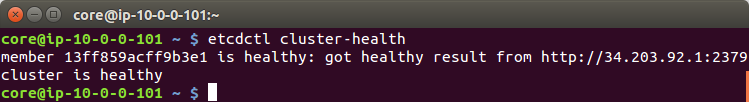
\includegraphics[width=0.8\textwidth]{images/figures/cluster-health-aws-1.png}
\caption{Comprobación de la salud del clúster con 1 máquina virtual.}
\end{figure}

Además se comprueba que la red virtual que une a los contenedores mediante direcciones IP virtuales funcione correctamente:

%= lang:bash
\begin{code}
$ sudo systemctl status flanneld
\end{code}

\begin{figure}[H]
\centering
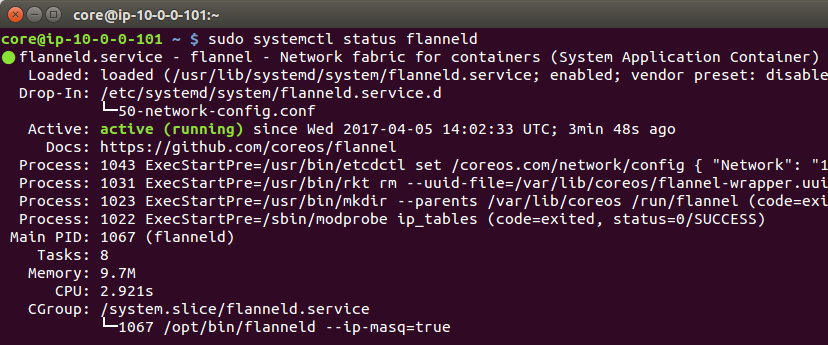
\includegraphics[width=0.8\textwidth]{images/figures/flanneld-aws-1.png}
\caption{Comprobación de la red virtual - \kode{core01}.}
\end{figure}

Por último se comprueba desde la consola de comandos que se puede acceder al servicio correctamente con el comando \kode{curl}:

%= lang:bash
\begin{code}
$ curl http://localhost:80 | tail -n 15
\end{code}

\begin{figure}[H]
\centering
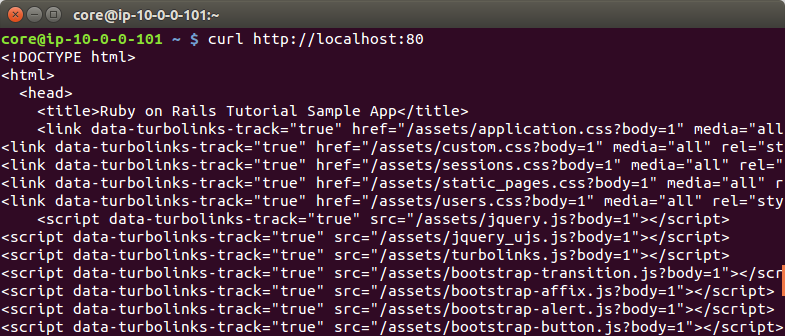
\includegraphics[width=0.7\textwidth]{images/figures/curl-aws-1.png}
\caption{Acceso al servicio por consola de comandos - \kode{core01}.}
\end{figure}

Además, se utiliza la IP elástica para acceder a través del navegador web:

\begin{figure}[H]
\centering
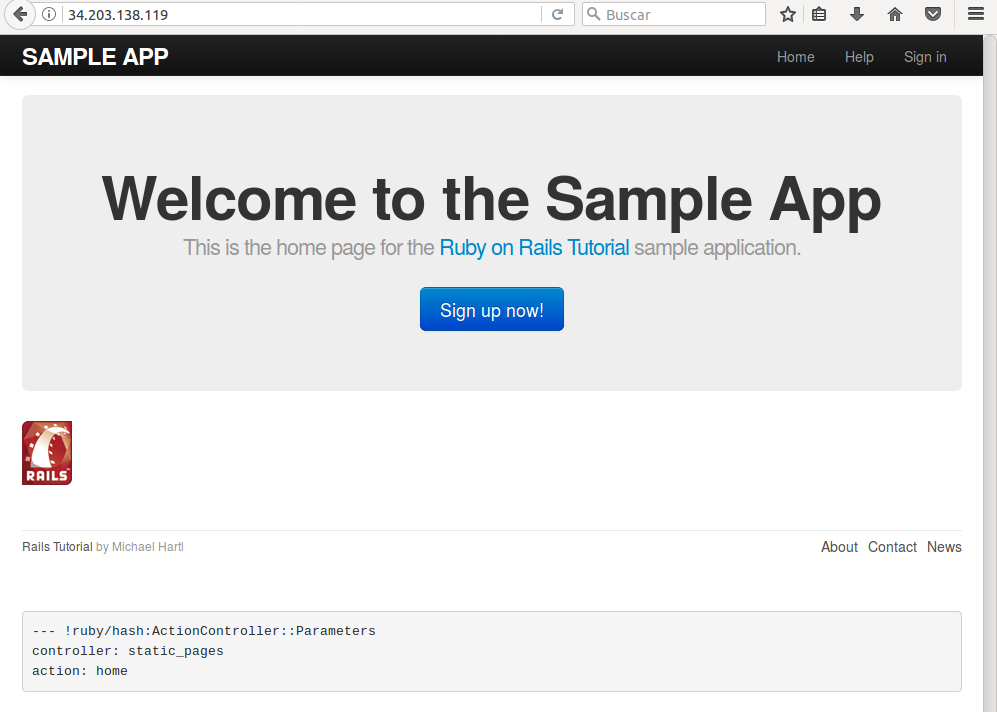
\includegraphics[width=0.7\textwidth]{images/figures/access-aws-1.png}
\caption{Acceso al servicio por el navegador web - \kode{core01}.}
\end{figure}

Desde la consola de AWS se puede apreciar dicha instancia:

\begin{figure}[H]
\image{images/figures/aws-console-1.png}
\caption{Consola AWS EC2 Instances - \kode{core-01}.}
\end{figure}

Para eliminar la infraestructura desplegada, así como los recursos asociados a ella, se ejecuta lo siguiente:

%= lang:bash
\begin{code}
$ vagrant destroy core-01 -f
\end{code}

\subsection{Despliegue de tres instancias}

Para poder realizar un despliegue de un clúster con varias máquinas virtuales se cambia el valor de la variable \kode{num\_instances} a 3. Este cambio se realiza tanto en \kode{cloud-config} como en \kode{config.rb}. En cuanto al servicio, lo que se consigue es tener en cada una de las instancias una copia del mismo.

A continuación se despliega esta infraestructura:

%= lang:bash
\begin{code}
$ vagrant up --provider=aws
\end{code}

Ahora se prueba, desde el sistema anfitrión, que la salud del clúster es positiva en todas las máquinas:

%= lang:bash
\begin{code}
$ for i in 1 2 3; do vagrant ssh core-0$i -c 'etcdctl cluster-health'; done
\end{code}

\begin{figure}[H]
\centering
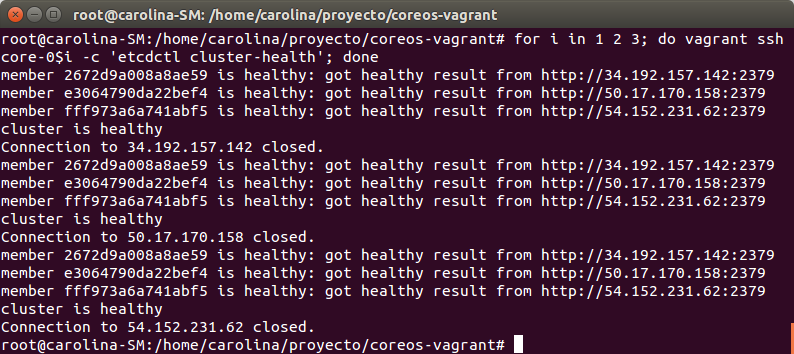
\includegraphics[width=0.8\textwidth]{images/figures/cluster-health-aws-3.png}
\caption{Comprobación de la salud del clúster en \kode{core-01}, \kode{core-02} y \kode{core-03}.}
\end{figure}

Además, se comprueba que la red virtual que une a los contenedores mediante direcciones IP virtuales funciona correctamente. En la siguiente imagen se puede apreciar, aunque el resultado del comando no devuelva colores, que el estado está activo y en ejecución:

%= lang:bash
\begin{code}
$ for i in 1 2 3; do vagrant ssh core-0$i -c 'sudo systemctl flanneld \
  | head -n16'; done
\end{code}

\begin{figure}[H]
\centering
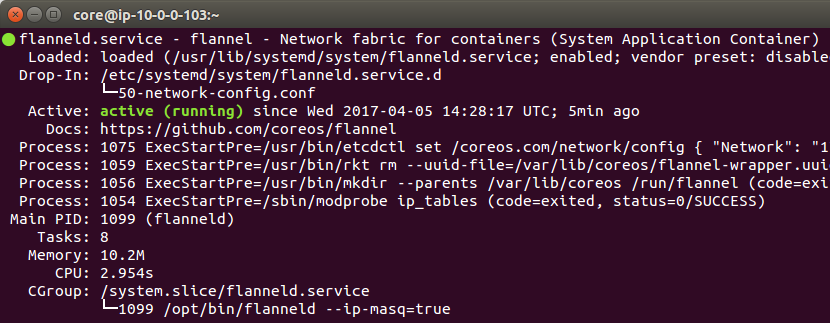
\includegraphics[width=0.8\textwidth]{images/figures/flanneld-aws-3.png}
\caption{Comprobación de la red virtual en \kode{core-01}, \kode{core-02} y \kode{core-03}.}
\end{figure}

Para probar que las máquinas virtuales tienen conexión con los contenedores de otras máquinas virtuales se obtiene, en primer lugar, la dirección IP del contenedor \kode{some-postgres} de la máquina virtual \kode{core-03}:

%= lang:bash
\begin{code}
$ docker inspect some-postgres
\end{code}

\begin{figure}[H]
\centering
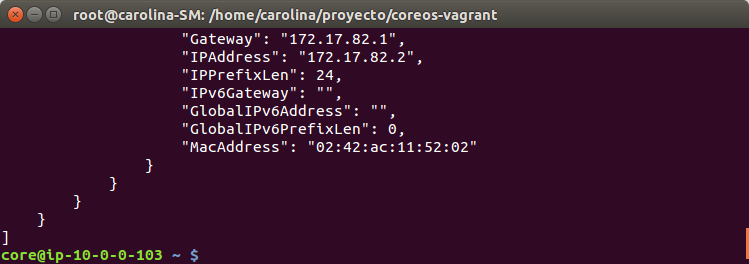
\includegraphics[width=0.8\textwidth]{images/figures/docker-inspect-3.png}
\caption{Obtención de la dirección IP de un contenedor en core-03.}
\end{figure}

Luego se prueba que haya conexión desde la máquina virtual \kode{core-01}:

\begin{figure}[H]
\centering
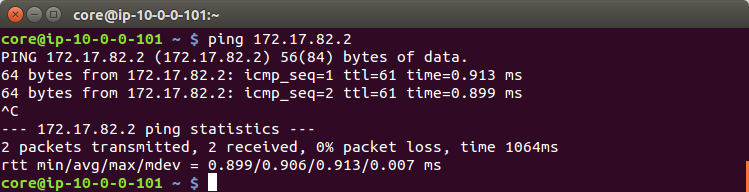
\includegraphics[width=0.8\textwidth]{images/figures/ping-1.png}
\caption{Prueba de conexión a un contenedor de core-03 desde core-01.}
\end{figure}

Por último se comprueba desde la consola de comandos que se puede acceder al servicio correctamente con el comando \kode{curl}. 

%= lang:bash
\begin{code}
$ for i in 1 2 3; do vagrant ssh core-0$i -c 'curl http://localhost:80 \
  | tail -n 15'; done
\end{code}

\begin{figure}[H]
\centering
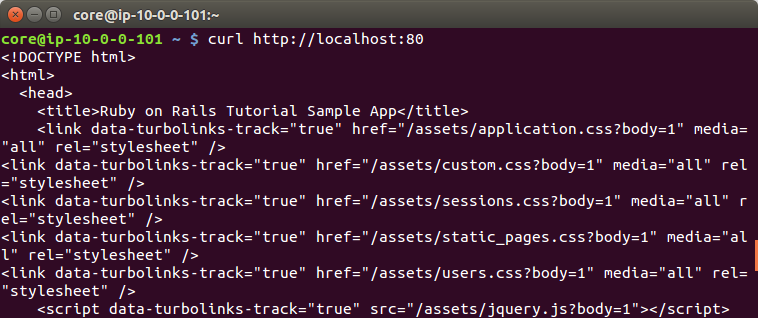
\includegraphics[width=0.8\textwidth]{images/figures/curl-aws-3.png}
\caption{Acceso al servicio por consola de comandos en \kode{core-01}, \kode{core-02} y \kode{core-03}.}
\end{figure}

Además, se utiliza la IP elástica de las instancias para acceder a través del navegador web:

\begin{figure}[H]
\centering
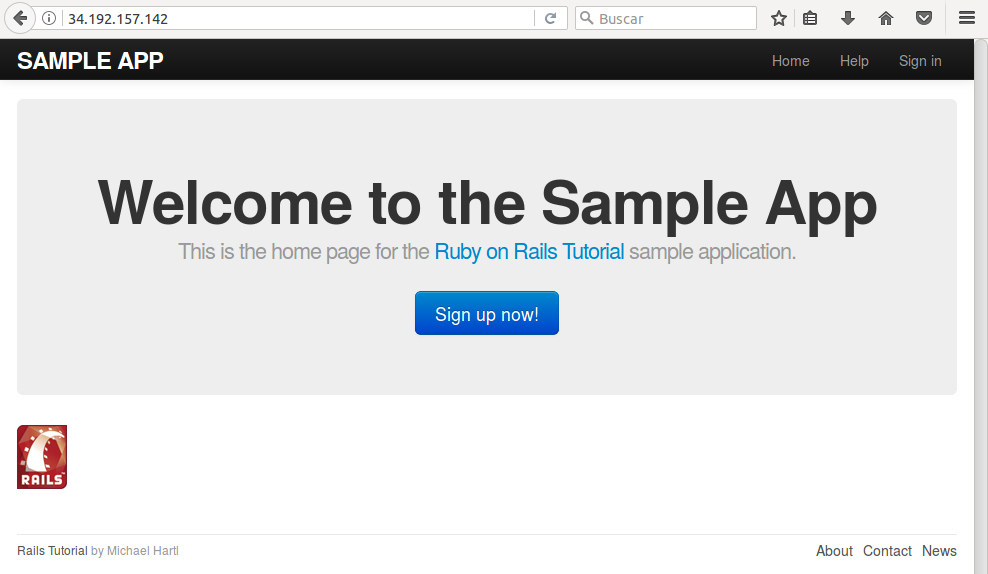
\includegraphics[width=0.7\textwidth]{images/figures/nav-1.png}
\caption{Acceso al servicio por el navegador web desde \kode{core-01}.}
\end{figure}

\begin{figure}[H]
\centering
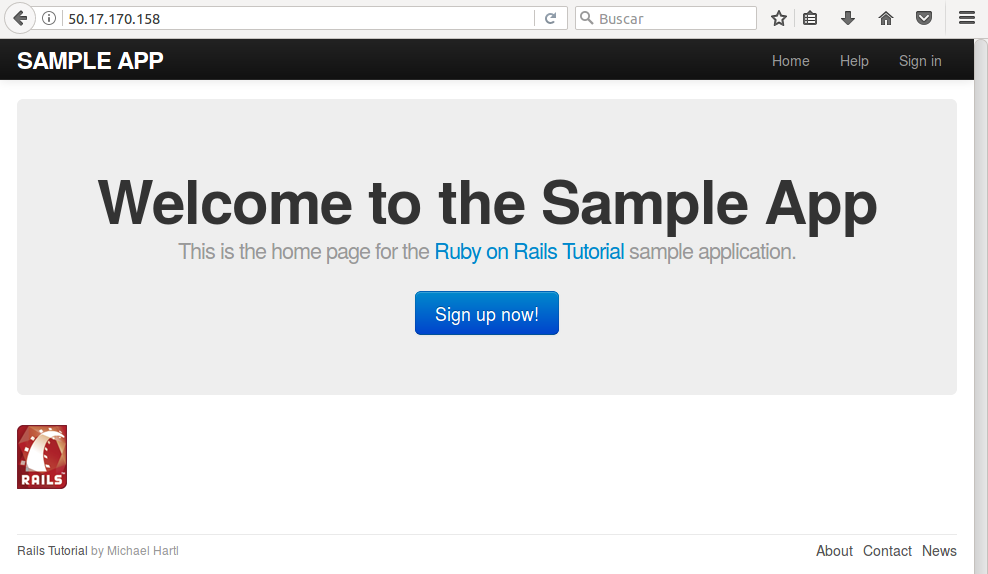
\includegraphics[width=0.7\textwidth]{images/figures/nav-2.png}
\caption{Acceso al servicio por el navegador web desde \kode{core-02}.}
\end{figure}

\begin{figure}[H]
\centering
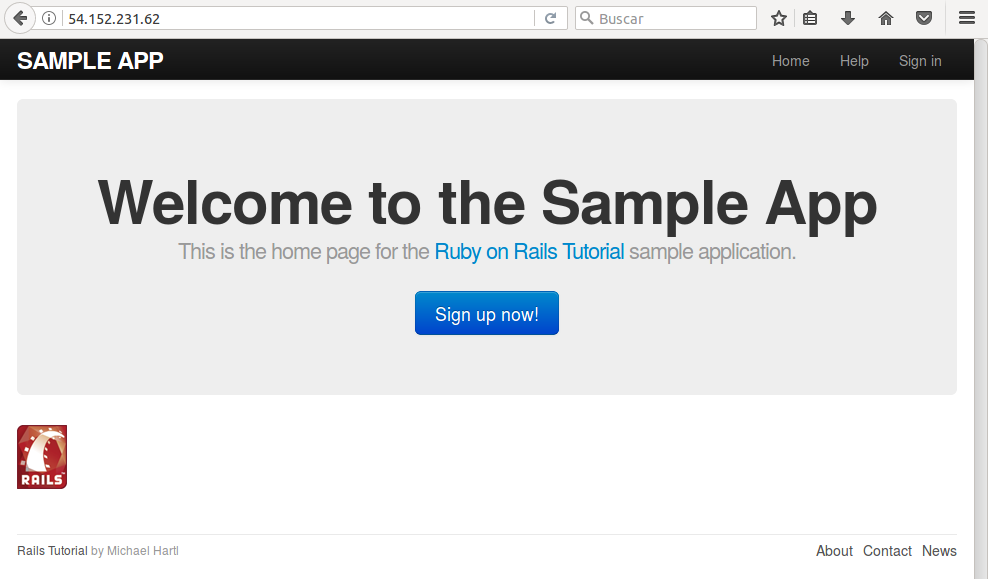
\includegraphics[width=0.7\textwidth]{images/figures/nav-3.png}
\caption{Acceso al servicio por el navegador web desde \kode{core-03}.}
\end{figure}

Desde la consola de AWS se pueden apreciar las 3 instancias y algunas de sus características con las que se ha trabajado:

\begin{figure}[H]
\image{images/figures/aws-console-3.png}
\caption{Consola AWS EC2 Instances - \kode{core-01}, \kode{core-02} y \kode{core-03}.}
\end{figure}

\subsection{Cambio de las unidades systemd a fleet}

Hasta ahora las unidades de servicio se han configurado globalmente en la sección propia de systemd. Con la intención de mejorar la distribución de la infraestructura se va a pasar a tratar a las unidades de servicio \kode{volume-public.service}, \kode{postgresql.service}, \kode{app-job.service}, \kode{app-task.service} y \kode{nginx.service} como unidades fleet. Para ello es necesario que los servicios sean especificados como ficheros a escribir en el sistema, concretamente se van a situar en la ruta \kode{/home/core/}. La sección \kode{[Install]} se cambia por la propia a fleet, \kode{X-Fleet}. Aquí se especificará el parámetro \kode{Global} que programa la unidad en todos los agentes del clúster de forma que desde cada una de las instancias que lo componen se puedan ver todos los servicios que hay en todas ellas. Luego se crean los servicios \kode{fleet-volume-public.service}, \kode{fleet-postgresql.service}, \kode{fleet-app-job.service}, \kode{fleet-app-task.service} y \kode{fleet-nginx.service} como unidades systemd que se van a encargar de indicar a fleet que ha de empezar los servicios pasados como ficheros. 

De esta manera, continuando con el clúster de 3 instancias, se cambia el fichero \kode{user-data.sampleapp-aws} por lo siguiente:

\begin{codelisting}
\label{code:vagrantfile2}
\codecaption{Fichero \kode{user-data.sampleapp-aws}}
%= lang:yaml
\begin{code}
#cloud-config
---
write_files:
  - path: "/etc/postgres-credentials.env"
    permissions: "0644"
    content: |
      POSTGRES_USER=postgres
      POSTGRES_PASSWORD=postgres
  - path: "/etc/nginx.conf"
    permissions: "0644"
    content: |
      server {
        listen 80;
        root /usr/src/app/public;
        location / {
          proxy_set_header X-Forwarded-For $proxy_add_x_forwarded_for;
          proxy_set_header Host $http_host;
          proxy_redirect off;
          try_files $uri /page_cache/$uri /page_cache/$uri.html @app;
        }
        location @app{
          proxy_pass http://app:9292;
          break;
        }
      }
  - path: "/home/core/volume-public.service"
    permissions: "0644"
    content: |
      [Unit] 
      Description= volume-public share between some-postgres, app-job, app-task 
                   and some-nginx 
      After=docker.service
      Requires=docker.service
      [Service] 
      TimeoutStartSec=0 
      ExecStart=/usr/bin/docker volume create --name volume-public
      [X-Fleet]
      Global=true
  - path: "/home/core/postgresql.service"
    permissions: "0644"
    content: |
      [Unit] 
      Description=PostgreSQL database 
      After=docker.service volume-public.service
      Requires=docker.service volume-public.service
      [Service] 
      TimeoutStartSec=0
      EnvironmentFile=/etc/postgres-credentials.env
      ExecStartPre=-/usr/bin/docker kill some-postgres 
      ExecStartPre=-/usr/bin/docker rm some-postgres 
      ExecStartPre=/usr/bin/docker pull postgres 
      ExecStart=/usr/bin/docker run --rm --name some-postgres \
      -e "POSTGRES_USER=${POSTGRES_USER}" \
      -e "POSTGRES_PASSWORD=${POSTGRES_PASSWORD}" \
      -v "volume-public:/var/lib/postgresql" -p "5432:5432" postgres 
      ExecStop=/usr/bin/docker stop some-postgres
      [X-Fleet]
      Global=true
  - path: "/home/core/app-job.service"
    permissions: "0644"
    content: |
      [Unit] 
      Description=executable app-job container that creates, migrates, seeds and 
                  populates the database
      After=docker.service volume-public.service postgresql.service
      Requires=docker.service volume-public.service postgresql.service
      [Service] 
      TimeoutStartSec=0 
      EnvironmentFile=/etc/postgres-credentials.env
      ExecStartPre=-/usr/bin/docker kill app-job 
      ExecStartPre=-/usr/bin/docker rm app-job 
      ExecStartPre=/usr/bin/docker pull carolina/sample_app_rails_4_image:latest 
      ExecStart=/usr/bin/docker run --rm --name app-job \
      -v "volume-public:/usr/src/app/public" --entrypoint "/setup.sh" \
      -e "POSTGRES_USER=${POSTGRES_USER}" \
      -e "POSTGRES_PASSWORD=${POSTGRES_PASSWORD}" \
      -w "/usr/src/app" --link "some-postgres:db" \
      carolina/sample_app_rails_4_image:latest
      [X-Fleet]
      Global=true
  - path: "/home/core/app-task.service"
    permissions: "0644"
    content: |
      [Unit] 
      Description=app-task container that runs the server puma
      After=docker.service volume-public.service postgresql.service 
            app-job.service
      Requires=docker.service volume-public.service postgresql.service 
               app-job.service
      [Service] 
      TimeoutStartSec=0 
      EnvironmentFile=/etc/postgres-credentials.env
      ExecStartPre=-/usr/bin/docker kill app-task 
      ExecStartPre=-/usr/bin/docker rm app-task
      ExecStartPre=/usr/bin/docker pull carolina/sample_app_rails_4_image:latest 
      ExecStart=/usr/bin/docker run --rm --name app-task \
      -e "POSTGRES_USER=${POSTGRES_USER}" \
      -e "POSTGRES_PASSWORD=${POSTGRES_PASSWORD}" \
      -w "/usr/src/app" -v "volume-public:/usr/src/app/public" \
      --link "some-postgres:db" \
      carolina/sample_app_rails_4_image:latest \
      /bin/bash -c "cp config/database.yml.postgresql config/database.yml \
                    && puma -p 9292"
      ExecStop=/usr/bin/docker stop app-task
      [X-Fleet]
      Global=true
  - path: "/home/core/nginx.service"
    permissions: "0644"
    content: |
      [Unit] 
      Description=some-nginx container that runs a reverse proxy server and a 
                  web server
      After=docker.service volume-public.service postgresql.service 
            app-job.service app-task.service
      Requires=docker.service volume-public.service postgresql.service 
               app-job.service app-task.service
      [Service] 
      TimeoutStartSec=0 
      ExecStartPre=-/usr/bin/docker kill some-nginx 
      ExecStartPre=-/usr/bin/docker rm some-nginx
      ExecStartPre=/usr/bin/docker pull nginx 
      ExecStart=/usr/bin/docker run --rm --name some-nginx \
      -v "/etc/nginx.conf:/etc/nginx/conf.d/default.conf" \
      -p "80:80" --link "app-task:app" \
      -v "volume-public:/usr/src/app/public" nginx 
      ExecStop=/usr/bin/docker stop some-nginx
      [X-Fleet]
      Global=true
coreos:
  etcd2:
    advertise-client-urls: http://$public_ipv4:2379
    initial-advertise-peer-urls: http://$private_ipv4:2380
    listen-client-urls: http://0.0.0.0:2379,http://0.0.0.0:4001
    listen-peer-urls: http://$private_ipv4:2380,http://$private_ipv4:7001
    discovery: https://discovery.etcd.io/558211c45a44606538213eddb032abc3
  fleet:
    public-ip: "$public_ipv4"
  flannel:
    interface: "$private_ipv4"
  units:
  - name: etcd2.service
    command: start
  - name: fleet.service
    command: start
    enable: true
  - name: flanneld.service
    drop-ins:
    - name: 50-network-config.conf
      content: |
        [Service]
        ExecStartPre=/usr/bin/etcdctl set /coreos.com/network/config 
                   '{ "Network": "172.17.0.0/16", "Backend": { "Type": "udp" } }'
    command: start
    enable: true
  - name: docker-tcp.socket
    command: start
    enable: true
    content: |
      [Unit]
      Description=Docker Socket for the API
      [Socket]
      ListenStream=2375
      Service=docker.service
      BindIPv6Only=both
      [Install]
      WantedBy=multi-user.target
  - name: fleet-volume-public.service
    command: start
    content: |
      [Unit]
      Description=Start volume-public.service using fleet
      [Service]
      ExecStart=/usr/bin/fleetctl start /home/core/volume-public.service
  - name: fleet-postgresql.service
    command: start
    content: |
      [Unit]
      Description=Start postgresql.service using fleet
      [Service]
      ExecStart=/usr/bin/fleetctl start /home/core/postgresql.service
  - name: fleet-app-job.service
    command: start
    content: |
      [Unit]
      Description=Start app-job.service using fleet
      [Service]
      ExecStart=/usr/bin/fleetctl start /home/core/app-job.service
  - name: fleet-app-task.service
    command: start
    content: |
      [Unit]
      Description=Start app-task.service using fleet
      [Service]
      ExecStart=/usr/bin/fleetctl start /home/core/app-task.service
  - name: fleet-nginx.service
    command: start
    content: |
      [Unit]
      Description=Start nginx.service using fleet
      [Service]
      ExecStart=/usr/bin/fleetctl start /home/core/nginx.service
\end{code}
\end{codelisting}

Para comprobar que todo funciona se levanta la infraestructura:

%= lang:bash
\begin{code}
$ vagrant up --provider=aws
\end{code}

La infraestructura desplegada es la siguiente:

\begin{figure}[H]
\image{images/figures/aws-console-fleet.png}
\caption{Consola AWS EC2 Instances - \kode{core-01}, \kode{core-02} y \kode{core-03}.}
\end{figure}

Una vez terminado, gracias al uso del parámetro \kode{Global=true} bastará con entrar en la máquina \kode{core-01} para comprobar que las unidades funcionan correctamente:

%= lang:bash
\begin{code}
$ vagrant ssh core-01
# fleetctl list-units
\end{code}

\begin{figure}[H]
\centering
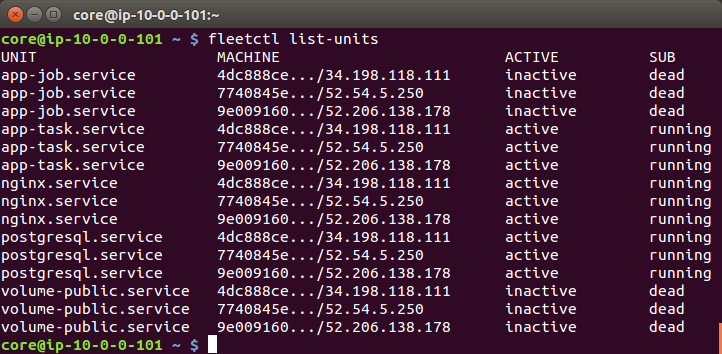
\includegraphics[width=0.8\textwidth]{images/figures/fleetctl-list-units.png}
\caption{Listado de unidades fleet en cada una de las máquinas.}
\end{figure}

Como se puede apreciar, cada una de las máquinas, con sus relativas direcciones IP, tiene una copia de cada servicio. Las unidades \kode{app-job.service} y \kode{volume-public.service} aparecen inactivas porque se tratan de contenedores ejecutables, cuando acaban su cometido terminan.

Además, se comprueba que la actividad sigue siendo correcta:

%= lang:bash
\begin{code}
$ for i in 1 2 3; do vagrant ssh core-0$i -c 'curl http://localhost:80 \
  | tail -n 15'; done
\end{code}

\begin{figure}[H]
\centering
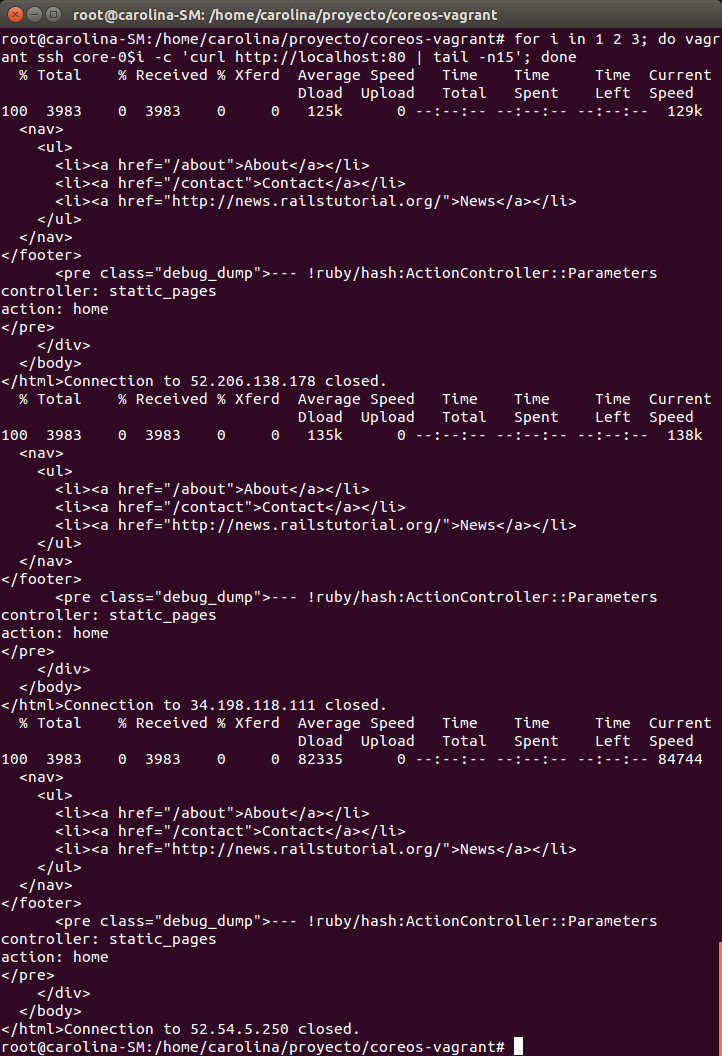
\includegraphics[width=0.8\textwidth]{images/figures/curl-fleet.png}
\caption{Acceso al servicio por consola de comandos en \kode{core-01}, \kode{core-02} y \kode{core-03}.}
\end{figure}

\subsection{Configuración DNS usando SkyDNS}

Con el objetivo de aislar la base de datos en una sola máquina se va a hacer uso de un servidor de sistema de nombres de dominio (DNS). Este servidor es necesario puesto que los contenedores \kode{app-job}, encargado de crear, migrar y poblar la base de datos, y \kode{app-task}, el propio servicio web, necesitan acceder al contenedor \kode{some-postgres}. Este contenedor, al no estar alojado en la misma máquina, tendrá que ser registrado en el servidor DNS para que pueda ser descubierto desde las otras máquinas. Así, los contenedor \kode{app-job} y \kode{app-task} resolverán la base de datos mediante dicho servidor DNS, que tendrá presencia en todas las máquinas como un nuevo contenedor, llamado \kode{skydns}. El servidor DNS a usar es SkyDNS, servicio distribuido para el anuncio y el descubrimiento de servicios construidos sobre etcd. De está manera crea registros en etcd y los lee desde el mismo sitio. Se trata de un proyecto de código abierto que puede ser encontrado en GitHub, bajo el repositorio \kode{skynetservices/skydns}\footnotettt{SkyDNS}{https://github.com/skynetservices/skydns}.

Así, el primer paso consistirá en la división de la infraestructura de forma que los contenedores \kode{volume-public}, \kode{app-job}, \kode{app-task} y \kode{some-ningx} sean creados en la máquina \kode{core-01}. Por otro lado, el contenedor \kode{some-postgres} será creado en la máquina \kode{core-02}. Esto se consigue usando la opción \textit{metadata} presente en las unidades fleet. Para especificarlo es necesario añadir al fichero \kode{Vagrantfile} un metadato diferente para cada una de las máquinas, de manera que \kode{core-01} reciba \textit{compute=web} y \kode{core-02} \textit{compute=db}. Esto ha de ser añadido bajo la carga de cada una de las líneas que contiene el fichero \kode{user-data}, en el momento en que detecta la sección de configuración fleet, bajo coreos.

\begin{codelisting}
\label{code:vagrantfile2}
\codecaption{Fichero \kode{Vagrantfile}}
%= lang:ruby
\begin{code}
.
data = YAML.load(IO.readlines(CLOUD_CONFIG_PATH)[1..-1].join)
if data['coreos'].key? 'fleet' and i==1
  data['coreos']['fleet']['metadata'] = 'compute=web'
end
if data['coreos'].key? 'fleet' and i==2
 data['coreos']['fleet']['metadata'] = 'compute=db'
end
.
\end{code}
\end{codelisting}

Ahora será necesario añadir el metadato a los ficheros de las unidades de servicio pertenecientes a los contenedores nombrados. Para la máquina \kode{core-01} el parámetro \textit{MachineMetadata=compute=web} y en el fichero correspondiente a la base de datos el parámetro \textit{MachineMetadata=compute=db}, en la máquina \kode{core-02}. Ambos en la sección \textit{[X-Fleet]}.

Como el contenedor \kode{some-postgres} ya no se encontrará en la misma máquina que el resto de contenedores no es posible compartir el volumen \kode{volume-public} con ellos. Por lo tanto se eliminará en su definición el comando \textit{-v}, que permite exportarlo, así como su inclusión en los parámentros \textit{After} y \textit{Require}.

Lo siguiente será crear el contenedor que se corresponde con el servidor DNS, presente en todas las máquinas. Este último hecho es posible no añadiendo ningún metadato en la sección \textit{[X-Fleet]}. Para ello se escribe un nuevo fichero llamado \kode{/home/core/skydns.service} antes del fichero \kode{/home/core/volumen-public.service}. Además se le indica que será iniciado después de docker y etcd2. Luego se procede de la misma manera que con las otras unidades de servicio. Antes de comenzar el servicio borrará el contenedor si existe previamente y luego descargará la imagen desde DockerHub. Antes de empezar el servicio se establece la configuración de SkyDNS de forma que se especifica la dirección IP y puerto en la que debe escuchar, que será la local a la máquina por el puerto 53: \kode{0.0.0.0:53}. También se establece el dominio para el que es autoritario, escogiéndose \kode{sampleapp.local.}, y el tiempo de vida (TTL) de las respuestas a 30 segundos. A la hora de comenzar el servicio restará indicarle que las máquinas etcd se comunican para los clientes en la dirección IP privada en uso y puerto 2379. Como se trata de una unidad fleet, será necesario añadir el servicio global \kode{fleet-skydns.service} antes de \kode{fleet-volume-public.service} para comenzar el servicio. Así habrá que añadir lo siguiente a \kode{user-data.sampleapp.aws}.

\begin{codelisting}
\label{code:user-data-skydns}
\codecaption{Fichero \kode{user-data.sampleapp.aws}}
%= lang:yaml
\begin{code}
.
write_files:
.
  - path: "/home/core/skydns.service"
    permissions: "0644"
    content: |
      [Unit]
      Description=SkyDNS
      After=docker.service etcd2.service
      Requires=docker.service etcd2.service

      [Service]
      Restart=always
      TimeoutStartSec=0
      ExecStartPre=-/usr/bin/docker rm -f skydns
      ExecStartPre=/usr/bin/docker pull skynetservices/skydns
      ExecStartPre=/usr/bin/etcdctl set /skydns/config \
        '{"dns_addr":"0.0.0.0:53", "domain": "sampleapp.local.", "ttl":30}'
      ExecStart=/usr/bin/docker run --rm --name skydns \
        -e ETCD_MACHINES="http://$private_ipv4:2379" skynetservices/skydns
      ExecStop=-/usr/bin/docker stop skydns

      [X-Fleet]
      Global=true
.
coreos:
.
  units:
  .
  - name: fleet-skydns.service
    command: start
    content: |
      [Unit]
      Description=Start skydns.service using fleet

      [Service]
      ExecStart=/usr/bin/fleetctl start /home/core/skydns.service
.
\end{code}
\end{codelisting}

Como se dijo inicialmente, este servicio funciona mediante registros y lecturas. De esta manera, al fichero \kode{/home/core/postgresql.service} hay que añadirle el registro de la dirección IP del contenedor some-postgres para que pueda ser encontrado por los otros contenedores, desde las otras máquinas. Este registro ha de ser añadido después de que el contenedor esté en ejecución, por lo que se especificará como \textit{ExecStartPost} y se llevará a cabo una espera hasta que se cumpla tal condición. Los contenedores \kode{app-job} y \kode{app-task} necesitan resolverlo como \textit{db} que es el nombre escogido como adaptador de la base de datos. Sin embargo, \kode{app-job} también resuelve por \textit{some-postgres}, puesto que antes de comenzar sus tareas espera a que dicho contenedor esté activo en el puerto 5432. Teniendo en cuenta estas condiciones se realizan dos registros, el primero tipo nombre canónico (CNAME) de \textit{some-postgres.sampleapp.local.} a \textit{db.sampleapp.local.} y el segundo tipo dirección IP de \textit{db.sampleapp.local.} en dirección IP perteneciente al contenedor \kode{some-postgres}, indicándole que será accesible por el puerto 5432.

\begin{codelisting}
\label{code:user-data-skydns-postgresql}
\codecaption{Fichero \kode{user-data.sampleapp.aws}}
%= lang:yaml
\begin{code}
.
write_files:
.
  - path: "/home/core/postgresql.service"
    .
      [Service]
      .
      ExecStartPost=/bin/bash -c 'while ! \
        [ $(/usr/bin/docker inspect -f ="{{.State.Running}}" some-postgres) \
        == "=true" ]; do sleep 1; done; \
        /usr/bin/etcdctl set /skydns/local/sampleapp/some-postgres \
        "{ \\"host\\": \\"db.sampleapp.local.\\"}" ; \
        /usr/bin/etcdctl set /skydns/local/sampleapp/db \
        "{ \\"host\\": \\"$(/usr/bin/docker inspect -f \
        "{{ .NetworkSettings.IPAddress }}" some-postgres)\\" , \\"port\\":5432}"'
.
\end{code}
\end{codelisting}

Referente a los contenedores \kode{app-job} y \kode{app-task} habrá que eliminar la opción \textit{--link} y utilizar las opciones \textit{--dns} que apuntará a la dirección IP del contenedor \kode{skydns} y \textit{--dns-search} donde se especifica el dominio trabajado \textit{sampleapp.local} para poder resolver por \textit{db} y \textit{some-postgres} sin especificar el dominio. Dichas modificaciones dejan la sección \textit{ExecStart} de ambas unidades de servicio de la siguiente forma:

\begin{codelisting}
\label{code:user-data-skydns-app}
\codecaption{Fichero \kode{user-data.sampleapp.aws}}
%= lang:yaml
\begin{code}
.
write_files:
.
  - path: "/home/core/app-job.service"
    .
      [Service]
      .
      ExecStart=/bin/bash -c 'usr/bin/docker run --rm --name app-job \
      -v "volume-public:/usr/src/app/public" --entrypoint "/setup.sh" \
      -e "POSTGRES_USER=${POSTGRES_USER}" \
      -e "POSTGRES_PASSWORD=${POSTGRES_PASSWORD}" \
      -w "/usr/src/app" --dns $(/usr/bin/docker inspect \
      -f "{{ .NetworkSettings.IPAddress }}" skydns) \
      --dns-search "sampleapp.local" carolina/sample_app_rails_4_image:latest'
      .
  - path: "/home/core/app-task.service"
    .
      [Service]
      .
      ExecStart=/bin/bash -c 'usr/bin/docker run --rm --name app-task \
      -e "POSTGRES_USER=${POSTGRES_USER}" \
      -e "POSTGRES_PASSWORD=${POSTGRES_PASSWORD}" \
      -w "/usr/src/app" -v "volume-public:/usr/src/app/public" \
      --dns $(/usr/bin/docker inspect \
      -f "{{ .NetworkSettings.IPAddress }}" skydns) \
      --dns-search "sampleapp.local" carolina/sample_app_rails_4_image:latest \
      /bin/bash \ -c "cp config/database.yml.postgresql config/database.yml && \
      puma -p 9292"'
      .
\end{code}
\end{codelisting}

Además habrá que quitar de las secciones \textit{After} y \textit{Requires} el servicio \kode{postgresql.service} en todos los servicios. Así como añadir \kode{skydns.service} antes de \kode{volume-public.service} en todas las unidades de servicio.

A continuación se desplega la infraestructura para poder realizar pruebas de funcionamiento:

%= lang:bash
\begin{code}
$ vagrant up --provider=aws
\end{code}

En primer lugar se comprueba que el clúster sea saludable, contemplado por todas las máquinas:

%= lang:bash
\begin{code}
$ for i in 1 2 3; do vagrant ssh core-0$i -c 'etcdctl cluster-health'; done
\end{code}

\begin{figure}[H]
\centering
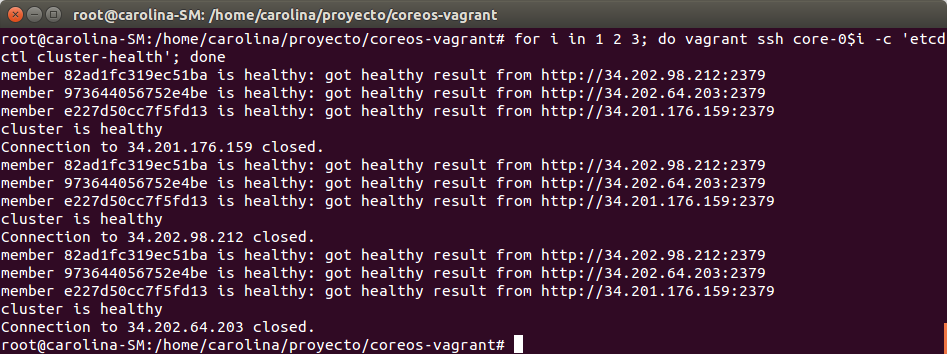
\includegraphics[width=0.85\textwidth]{images/figures/skydns-health.png}
\caption{Salud del clúster contemplada por las 3 máquinas.}
\end{figure}

Luego se listan las máquinas y se comprueba que han recibido el metadato pertinente:

%= lang:bash
\begin{code}
for i in 1 2 3; do vagrant ssh core-0$i -c 'fleetctl list-machines'; done
\end{code}

\begin{figure}[H]
\centering
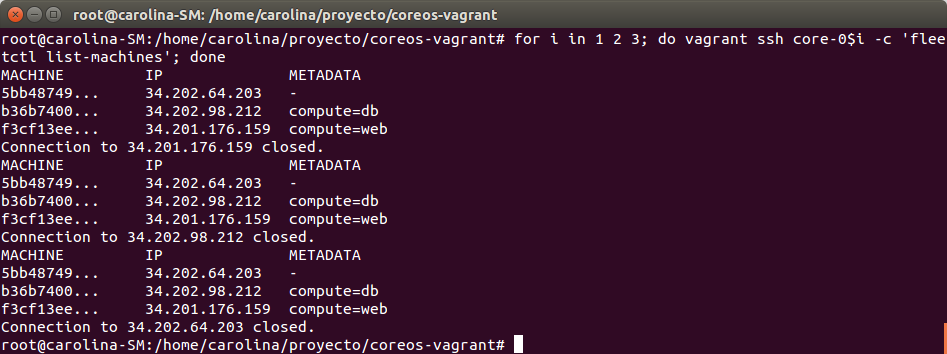
\includegraphics[width=0.85\textwidth]{images/figures/skydns-machines.png}
\caption{Información de las máquinas contemplada por las 3 instancias.}
\end{figure}

También se comprueba que las unidades de servicio se han creado donde se indicó:
%= lang:bash
\begin{code}
$ for i in 1 2 3; do vagrant ssh core-0$i -c 'fleetctl list-units'; done
\end{code}

\begin{figure}[H]
\centering
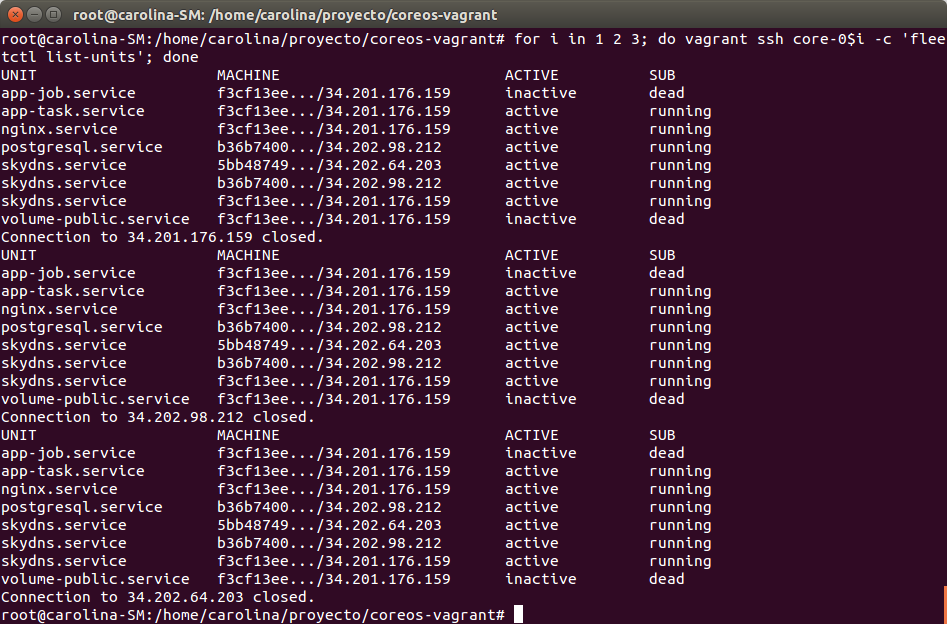
\includegraphics[width=0.85\textwidth]{images/figures/skydns-units.png}
\caption{Información de las unidades contemplada por las 3 máquinas.}
\end{figure}

Se comprueba que los registros se hayan establecido correctamente:

%= lang:bash
\begin{code}
$ for i in 1 2 3; do vagrant ssh core-0$i -c '/usr/bin/etcdctl get \
  /skydns/local/sampleapp/db; \
  /usr/bin/etcdctl get /skydns/local/sampleapp/some-postgres '; done
\end{code}

\begin{figure}[H]
\centering
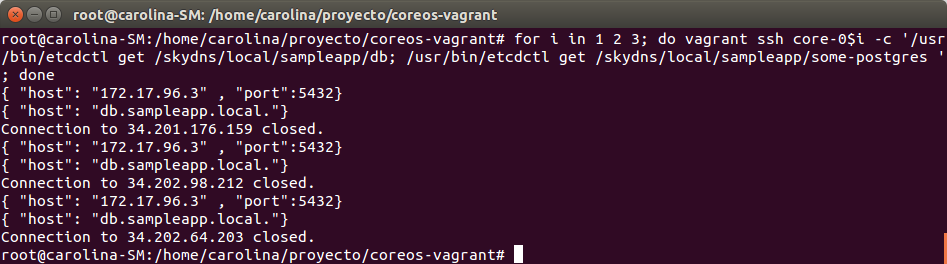
\includegraphics[width=0.85\textwidth]{images/figures/skydns-gets.png}
\caption{Lectura de los registros en SkyDNS contemplada por las 3 máquinas.}
\end{figure}

La máquina \kode{core-01} resuelve tanto \textit{db} como \textit{some-postgres}:

%= lang:bash
\begin{code}
docker exec -it app-task sh -c 'ping -c 1 db'
docker exec -it app-task sh -c 'ping -c 1 some-postgres'
\end{code}

\begin{figure}[H]
\centering
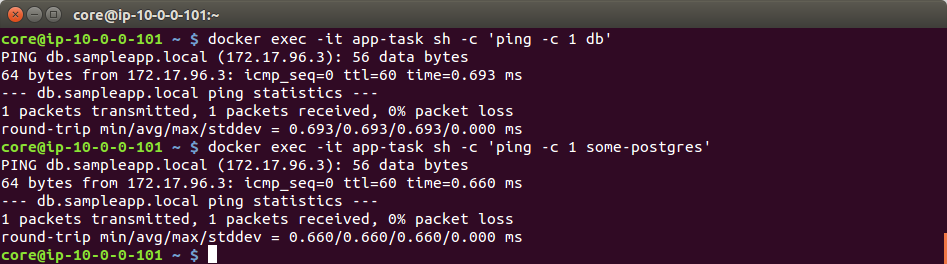
\includegraphics[width=0.85\textwidth]{images/figures/skydns-ping.png}
\caption{Conexión a \textit{db} como \textit{some-postgres} desde \kode{app-task}.}
\end{figure}

De esta manera, los registros ingresados han quedado como se pretendía:

%= lang:bash
\begin{code}
docker exec -it skydns sh -c 'dig @localhost db.sampleapp.local. A'
\end{code}

\begin{figure}[H]
\centering
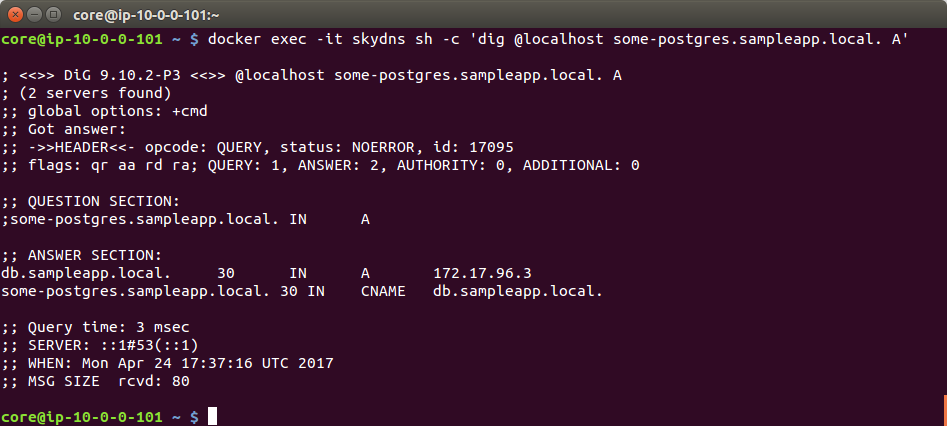
\includegraphics[width=0.85\textwidth]{images/figures/skydns-dig.png}
\caption{Registros DNS desde el contenedor \kode{skydns}.}
\end{figure}

Así, el servicio funciona correctamente en la máquina \kode{core-01}:
%= lang:bash
\begin{code}
$ for i in 1 2 3; do vagrant ssh core-0$i -c 'curl http://localhost:80 | \
  tail -n 15'; done
\end{code}

\begin{figure}[H]
\centering
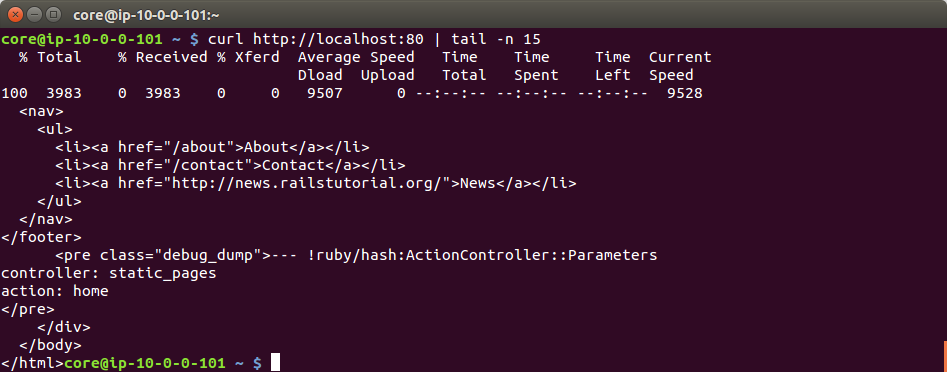
\includegraphics[width=0.85\textwidth]{images/figures/skydns-curl.png}
\caption{Conexión al servicio mediante consola desde \kode{core-01}.}
\end{figure}

Y mediante la web y la dirección IP elástica se ingresa con uno de los usuarios poblados en la base de datos, comprobando que sigue funcionando correctamente hasta este punto:

\begin{figure}[H]
\centering
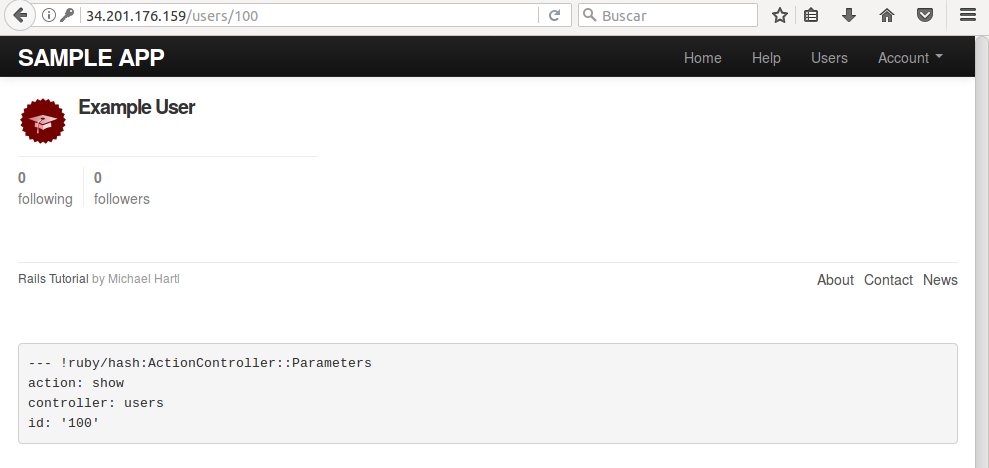
\includegraphics[width=0.85\textwidth]{images/figures/skydns-web.png}
\caption{Inicio de sesión con uno de los usuarios mediante navegador web desde la dirección IP elástica de \kode{core-01}.}
\end{figure}

\subsection{Balanceo de carga con Nginx usando Confd}

Con el propósito de implementar la infraestructura final, en la que en cada una de las máquinas que conforma el clúster hay un servidor de la aplicación, en la primera máquina se sitúa el proxy que balanceará la carga entre los anteriores y en la segunda máquina se encontrará la base de datos a la que acudirán los servidores de aplicación se van a realizar los siguientes cambios. 

En primer lugar, al no encontrarse los distintos contenedores en la misma máquina la opción de tener el volumen Docker \kode{volume-public} compartido entre ellos no es posible en la manera en la que se ha ido haciendo, así que se elimina su definición en el fichero \kode{user-data.sampleapp.aws}, en \kode{/home/core/volume-public.service}, su inclusión en los parámetros \textit{After} y \textit{Requires} en los servicios que lo implementan, el parámetro \textit{-v} que lo exporta en los contenedores \kode{app-job}, \kode{app-task} y \kode{some-nginx}, así como la unidad global \kode{fleet-volume-public.service}.

El despliegue de la infraestructura será controlado, una vez más, con metadatos. Para ello se mantiene a la máquina \kode{core-02} con el metadato \textit{compute=db} y se modifica en el fichero \kode{Vagrantfile}, bajo la carga de la línea que contiene la sección de configuración fleet en el fichero \kode{user-data}, el metadato para la máquina \kode{core-01}, cambiándolo por \textit{compute=proxy}.

\begin{codelisting}
\label{code:vagrantfile2}
\codecaption{Fichero \kode{Vagrantfile}}
%= lang:ruby
\begin{code}
.
data = YAML.load(IO.readlines(CLOUD_CONFIG_PATH)[1..-1].join)
if data['coreos'].key? 'fleet' and i==1
 data['coreos']['fleet']['metadata'] = 'compute=proxy'
end
.
\end{code}
\end{codelisting}

Ahora será necesario modificar el metadato de la unidad de servicio \kode{postgresql.service} a \textit{MachineMetadata=compute=proxy}, en la sección \textit{[X-Fleet]}. Además, se quita  en las unidades de servicio \kode{app-job.service} y \kode{app-task.service}, para que sean ubicadas en cada una de las máquinas que conforme el clúster.

Como el servicio \kode{nginx.service} tendrá que balancear la carga entre los distintos servidores web disponibles, será necesario que el servidor \kode{app-task} se registre tras crearse. Este registro se va a realizar en etc2, por lo tanto, éste se añade en los parámetros \textit{After} y \textit{Requires} como \kode{etcd2.service} tras \kode{docker.service}. Así, el registro se añade en la sección \textit{ExecStartPost} con clave \kode{/services/app/<dirección IP de la máquina en la que se encuentra>} y valor correspondiente con la dirección IP del contenedor y puerto 9292, pues se hace referencia al servidor puma. Para poder interpretar la dirección IP de la máquina es necesario que en la definición de esta unidad de servicio se indique el fichero de variables de entorno \kode{/etc/environment}. Esto permitirá tener tantas entradas \kode{/services/app/*} como máquinas en las que se ejecute hayan. También es importante añadir que cuando el contenedor deje de ejecutarse dicho registro sea borrado.

\begin{codelisting}
\label{code:execstartpost-app-task}
\codecaption{Fichero \kode{user-data.sampleapp.aws}}
%= lang:yaml
\begin{code}
.
write_files:
.
  - path: "/home/core/app-task.service"
    .
    [Service] 
      .     
      EnvironmentFile=/etc/environment
      .
      ExecStartPost=/bin/bash -c 'while ! [ $(/usr/bin/docker inspect \
      -f ="{{.State.Running}}" app-task) == "=true" ]; do sleep 1; done; \
      etcdctl set /services/app/${COREOS_PRIVATE_IPV4} $(/usr/bin/docker \
      inspect -f "{{ .NetworkSettings.IPAddress }}" app-task):9292'
      ExecStop=/usr/bin/etcdctl rm /services/app/${COREOS_PRIVATE_IPV4}
      .
.
\end{code}
\end{codelisting}

Para que el servicio \kode{nginx.service} pueda registrar los servidores web puma se va a utilizar el servicio confd. Esta utilidad se encarga de controlar los cambios que se produzcan en etc2, vigilando las claves que se le indique. Cuando hay un nuevo registro o baja transfiere estos cambios a la configuración de nginx, por medio de una plantilla, modificando el fichero \kode{/etc/nginx.conf} del contenedor \kode{some-nginx}. Luego, hace efectivo el cambio reiniciando el servicio nginx. Este servicio puede ser encontrado en el repositorio \kode{kelseyhightower/confd}\footnotettt{confd}{https://github.com/kelseyhightower/confd} en GitHub, del que se hará una configuración especifica para este uso.

Como se pretende compartir el fichero de configuración \kode{nginx.conf} entre el contenedor \kode{some-nginx} y el futuro contenedor \kode{confd} se crea un volumen Docker, llamado \kode{conf-data}, que compartirá el directorio \kode{/etc/nginx} entre ambos. En su definición se indica requiere y ha de ser lanzado después del servicio \kode{docker.service}. Se indica que el servicio será de tipo \textit{oneshot}, lo que significa que el parámetro \textit{ExecStart} ha de ejecutarse solo una vez, sin reintentarlo. También se especifica la opción \textit{RemainAfterExit=yes} para que cuando el contenedor termine permanezca activo. Si el volumen existe en su lanzamiento se detiene y elimina. La imagen que se usa para el contenedor es la de nginx, para poder tener la misma disposición de directorios. Este volumen deberá ubicarse en la máquina \kode{core-01}, por lo que se le añade el metadato \kode{compute=proxy}. Además. será necesario crear la unidad global \kode{fleet-conf-data.service} que de comienzo a este servicio fleet.

\begin{codelisting}
\label{code:conf-data}
\codecaption{Fichero \kode{user-data.sampleapp.aws}}
%= lang:yaml
\begin{code}
.
write_files:
.
  - path: "/home/core/conf-data.service"
    permissions: "0644"
    content: |
      [Unit] 
      Description=conf data container to share files between confd and some-nginx
      After=docker.service
      Requires=docker.service
      [Service] 
      Type=oneshot
      RemainAfterExit=yes
      ExecStartPre=-/usr/bin/docker kill conf-data 
      ExecStartPre=-/usr/bin/docker rm conf-data
      ExecStartPre=/usr/bin/docker pull nginx 
      ExecStart=/usr/bin/docker run -v /etc/nginx --name conf-data nginx \
      echo "conf-data container created" 
      [X-Fleet]
      Global=true
      MachineMetadata=compute=proxy
  .
coreos:
  .
  units:
  .
  - name: fleet-conf-data.service
    command: start
    content: |
      [Unit]
      Description=Start conf-data.service using fleet
      [Service]
      ExecStart=/usr/bin/fleetctl start /home/core/conf-data.service
  .
\end{code}
\end{codelisting}

El servicio confd a implementar necesitará disponer de tres ficheros, que serán escritos en la máquina y exportados al contenedor a través del volumen \kode{conf-data}.

El primero de ellos es la plantilla \kode{nginx.conf.tmpl}, correspondiente a la configuración de nginx. Al incorporarlo a \kode{user-data.sampleapp.app} puede borrarse la definición del fichero \kode{/etc/nginx.conf}, presente en la sección \textit{write-files}. La información que se añade a la configuración que se ha trabajado anteriormente es la englobada en el bloque \textit{upstream}. Esta sección es utilizada para definir los servidores a los cuales nginx puede enviar peticiones. Nginx seleccionará uno de ellos dependiendo del método de distribución escogido, en este caso \textit{Round Robin}, del primero al último, que por defecto es el que se implementa. Mediante una plantilla en formato \textit{Go}, que permite gestionar contenido dinámico, se define este nuevo bloque, que ha de estar, a su vez, dentro del bloque \textit{http} y requiere la existencia del bloque \textit{events} para gestionar eventos, aunque no sea utilizado. Así, cuando confd analice etc2 en busca de cambios para las claves \kode{/services/app/*} sustituirá dinámicamente su contenido por las líneas \textit{server <dirección IP del contenedor \kode{app-task}>:9292}, en lugar de tener que definirlos estáticamente. Esta información será luego sustituida con el servidor escogido en la línea \textit{proxy\_pass http://app;}.

\begin{codelisting}
\label{code:nginx.conf.tmpl}
\codecaption{Fichero \kode{user-data.sampleapp.aws}}
%= lang:yaml
\begin{code}
.
write_files:
.
  - path: "/etc/nginx.conf.tmpl"
    permissions: "0644"
    content: |
      events {
      }
      http {
        upstream app {
        {{ range getvs "/services/app/*" }}
          server {{ . }};
        {{ end }}
        }

        server {
          listen 80;
          root /usr/src/app/public;
          location / {
            proxy_set_header X-Forwarded-For $proxy_add_x_forwarded_for;
            proxy_set_header Host $http_host;
            proxy_redirect off;
            try_files $uri /page_cache/$uri /page_cache/$uri.html @app;
          }
          location @app{
            proxy_pass http://app;
            break;
          }
        }
      }
.
\end{code}
\end{codelisting}

El siguiente, llamado \kode{nginx.toml}, representa el fichero de configuración de confd. Está escrito en formato TOML y permite comprobar el valor de las claves registradas bajo \kode{/services/app} y realizar la acción del cambio del archivo \kode{/etc/nginx/nginx.conf}, tomando como fuente la plantilla anterior, \kode{nginx.conf.tmpl}. Por último, el servicio confd ha de encargarse de reiniciar el servicio nginx. Para ello ejecuta el fichero \kode{/reload.sh}, un script que permitirá ejecutar una orden, mediante el comando curl, haciendo uso del socket de Docker, puesto que este servicio no estará instalado en el contenedor \kode{confd}. Esta orden hará que capture el identificador del contenedor \kode{some-nginx}, a través del lenguaje de gestión de flujos de datos JSON \textit{jq}, y mande a detener el proceso. 

\begin{codelisting}
\label{code:nginx.conf.tmpl}
\codecaption{Fichero \kode{user-data.sampleapp.aws}}
%= lang:yaml
\begin{code}
.
write_files:
.
  - path: "/home/core/reload.sh"
    permissions: "0644"
    content: |
      #!/bin/sh
      curl --unix-socket /var/run/docker.sock -XPOST \
      "http://v1.26/containers/$(curl --unix-socket /var/run/docker.sock \
      'http://v1.26/containers/json' | jq -r '.[] | \
       select(.Names[0] == "/some-nginx") .Id')/kill"
  - path: "/etc/nginx.toml"
    permissions: "0644"
    content: |
      [template]
      src = "nginx.conf.tmpl"
      dest = "/etc/nginx/nginx.conf"
      keys = [ "/services/app" ] 
      reload_cmd = "sh /reload.sh"
.
\end{code}
\end{codelisting}

Para poder disponer de una imagen Docker propia de confd, con una configuración determinada, se crea una nueva, llamada \kode{confd\_image}, a partir del fichero Dockerfile. Así, se utiliza una imagen Docker mínima basada en \textit{Alpine Linux}\footnotettt{Alpine Linux}{https://www.alpinelinux.org/about} con un índice de paquetes completo y solo 5 MB de tamaño, en su versión 3.3. Sobre esta imagen se instalarán los paquetes \textit{curl}, para poder hacer la recarga del servicio, y el \textit{jq}, para poder obtener el identificador del contenedor \kode{some-nginx}. Cuando están descargados se obtiene del repositorio GitHub comentado la herramienta confd, para sistemas Linux con CPUs AMD de 64 bits, se le dan permisos de lectura, escritura y ejecución al propietario en \kode{/usr/bin/confd} para poder realizar las operaciones y se limpia la memoria caché utilizada. Además, se añade el directorio vacío \kode{/etc/confd} que será utilizado para alojar los ficheros. Por último, se indica que una vez arrancado un contenedor con esta imagen, el servicio confd vigilará los cambios producidos en etc2, en todo el clúster, cada 5 segundos.

\begin{codelisting}
\label{code:dockerfile-confd}
\codecaption{Contenido de \kode{Dockerfile}}
%= lang:ruby
\begin{code}
FROM alpine:3.3
LABEL confd_image.version="0.1" confd_image.release-date="2017-05-02"
MAINTAINER Carolina Santana "c.santanamartel@gmail.com"
RUN apk add --update curl && apk add --update jq && \
    curl -o /usr/bin/confd -L https://github.com/kelseyhightower/confd/releases/
            download/v0.7.1/confd-0.7.1-linux-amd64 && \
    chmod 755 /usr/bin/confd && rm -rf /var/cache/apk/*
ADD etc/confd/ /etc/confd
CMD /usr/bin/confd -interval=5 -node=http://$COREOS_PRIVATE_IPV4:4001
\end{code}
\end{codelisting}

De esta manera, será necesario crear en local el directorio vacío \kode{etc/confd}, construir la imagen y subirla a DockerHub para poder usarla:

%= lang:bash
\begin{code}
$ mkdir etc/confd
$ docker login
$ docker build -t confd_image .
$ docker tag <image-id> carolina/confd_image:latest
$ sudo docker push carolina/confd_image
\end{code}

Cuando el proceso de subida ha terminado, se define el fichero \kode{/home/core/confd.service} que creará el contenedor \kode{confd}. Así, requiere y ha de ser creado tras los servicios \kode{docker.service}, \kode{etcd2.service}, pues leerá de él, y \kode{conf-data.service}. Se indica que comience automáticamente los intentos de ejecución de \textit{ExecStart} y se añade el fichero de variables de entorno \kode{/etc/environment} para que pueda conocer las direcciones IP de las máquinas que conforman el clúster. Si en el momento de ser lanzado ya existiera se manda a detener el proceso y se elimina el contenedor. Antes de crear el mismo se descarga la última versión de la imagen \kode{confd\_image}, si no se tiene. Además de pasarle la variable de entorno comentada, se exporta el socket de Docker, para poder hacer uso del mismo a la hora de ejecutar la recarga del servicio nginx y los tres archivos escritos, donde los destinos finales serán \kode{/etc/confd/templates/nginx.conf.tmpl}, \kode{/reload.sh} y \kode{/etc/confd/conf.d/nginx.toml}. Por último se añade el volumen \kode{conf-data}. Este contenedor deberá ubicarse en la máquina \kode{core-01}, por lo que se le añade el metadato \kode{compute=proxy}. También se crea la unidad global \kode{fleet-confd.service} que de comienzo a este servicio fleet.

\begin{codelisting}
\label{code:confd}
\codecaption{Fichero \kode{user-data.sampleapp.aws}}
%= lang:yaml
\begin{code}
.
write_files:
.
  - path: "/home/core/confd.service"
    permissions: "0644"
    content: |
      [Unit] 
      Description=confd container that updates nginx.conf file and kill 
                  some-nginx container to restart nginx service when detects
                  a new rails server has been registered
      After=docker.service etcd2.service conf-data.service
      Requires=docker.service etcd2.service conf-data.service
      [Service] 
      TimeoutStartSec=0 
      EnvironmentFile=/etc/environment
      ExecStartPre=-/usr/bin/docker kill confd 
      ExecStartPre=-/usr/bin/docker rm confd
      ExecStartPre=/usr/bin/docker pull carolina/confd_image:latest 
      ExecStart=/bin/bash -c '/usr/bin/docker run --rm --name confd \
      -e COREOS_PRIVATE_IPV4=${COREOS_PRIVATE_IPV4} \
      -v "/var/run/docker.sock:/var/run/docker.sock" \
      -v "/etc/nginx.conf.tmpl:/etc/confd/templates/nginx.conf.tmpl" \
      -v "/home/core/reload.sh:/reload.sh" \
      -v "/etc/nginx.toml:/etc/confd/conf.d/nginx.toml" \
      --volumes-from=conf-data carolina/confd_image '
      ExecStop=/usr/bin/docker stop confd
      [X-Fleet]
      Global=true
      MachineMetadata=compute=proxy
  .
coreos:
  .
  units:
  .
  - name: fleet-confd.service
    command: start
    content: |
      [Unit]
      Description=Start confd.service using fleet
      [Service]
      ExecStart=/usr/bin/fleetctl start /home/core/confd.service
  .
\end{code}
\end{codelisting}

En último lugar se realizan modificaciones en la definición del fichero \kode{/home/core/nginx.service} de manera que se especifique en las opciones \textit{After} y \textit{Requires} que requiere y ha de ir tras los servicios \kode{docker.service}, \kode{conf-data.service} y \kode{confd.service}. Como el servicio confd se encargará de detener el proceso de \kode{some-nginx} se añade la opción \textit{Restart=always} que, junto a la opción \textit{TimeoutStartSec=0} hará que la unidad de servicio vuelva a ejecutarse con la nueva configuración nginx. Además, en la creación del contenedor, \textit{ExecStart}, se elimina la opción \kode{--link app-task:app} y el fichero de configuración que se exportaba anteriormente \kode{-v /etc/nginx.conf:/etc/nginx/nginx.conf} y se añade la opción \kode{--volumes-from=conf-data}.

A continuación se despliega la infraestructura:

%= lang:bash
\begin{code}
$ . ~/.aws-credentials/aws-credentials
$ vagrant up --provider=aws
\end{code}

En primer lugar se comprueba la salud del clúster:

%= lang:bash
\begin{code}
$ for i in 1 2 3; do vagrant ssh core-0$i -c 'etcdctl cluster-health'; done
\end{code}

\begin{figure}[H]
\centering
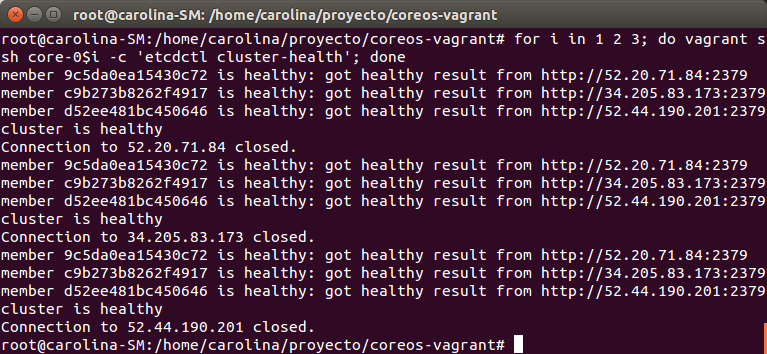
\includegraphics[width=0.7\textwidth]{images/figures/health-confd.png}
\caption{Salud del clúster contemplada por las 3 máquinas.}
\end{figure}

También, se visualizan las máquinas que conforman el clúster, con los metadatos asignados, así como las unidades fleet presentes en cada una de las máquinas:

%= lang:bash
\begin{code}
for i in 1 2 3; do vagrant ssh core-0$i -c 'fleetctl list-machines'; done
\end{code}

\begin{figure}[H]
\centering
\includegraphics[width=0.7\textwidth]{images/figures/machines-confd.png}
\caption{Información de las máquinas contemplada por las 3 máquinas.}
\end{figure}

%= lang:bash
\begin{code}
$ for i in 1 2 3; do vagrant ssh core-0$i -c 'fleetctl list-units'; done
\end{code}

\begin{figure}[H]
\centering
\includegraphics[width=0.7\textwidth]{images/figures/units-confd.png}
\caption{Información de las unidades fleet contemplada por las 3 máquinas.}
\end{figure}

Para continuar con las pruebas se escoge la máquina \kode{core-01}.

Se comprueban los registros existentes bajo la clave \kode{services/app/<dirección IP de \kode{app-task}>}. Las claves se averiguan con el comando \kode{etcdctl ls --recursive /services/app} y luego los valores con el comando \kode{etcdctl get /services/app/<dirección IP de \kode{app-task}>}:

\begin{figure}[H]
\centering
\includegraphics[width=0.7\textwidth]{images/figures/recursive-confd.png}
\caption{Obtención de claves y valores para \kode{services/app/<dirección IP de \kode{app-task}}.}
\end{figure}

Ahora que los contenedores \kode{app-task} se han registrado se puede comprobar como el servicio confd ha actualizado el fichero de configuración nginx, a medida que ha ido detectando cada uno de los tres. Esto es observado tanto desde los registros de operación del servicio \kode{confd.service} como entrando dentro del contenedor \kode{some-nginx} y viendo el contenido del fichero \kode{/etc/nginx/nginx.conf}:

%= lang:bash
\begin{code}
$ journalctl -u confd.service
\end{code}

\begin{figure}[H]
\centering
\includegraphics[width=0.8\textwidth]{images/figures/update-journal-confd.png}
\caption{Información de operaciones del contenedor \kode{confd} de actualización de la configuración nginx.}
\end{figure}

%= lang:bash
\begin{code}
$ docker exec -it some-nginx sh
# cat /etc/nginx/nginx.conf
\end{code}

\begin{figure}[H]
\centering
\includegraphics[width=0.7\textwidth]{images/figures/update-nginx-confd.png}
\caption{Fichero \kode{nginx.conf} actualizado.}
\end{figure}

Tras ver el orden en el que se han colocado las distintas direcciones IP de los contenedores \kode{app-task} puede conocerse de qué máquina proviene cada uno inspeccionando el contenedor en cada máquina:

%= lang:bash
\begin{code}
$ docker inspect app-task -f "{{ .NetworkSettings.IPAddress }}"
\end{code}

\begin{figure}[H]
\centering
\includegraphics[width=0.7\textwidth]{images/figures/IP1-confd.png}
\caption{Dirección IP del contenedor \kode{app-task} en la máquina \kode{core-01}.}
\end{figure}

\begin{figure}[H]
\centering
\includegraphics[width=0.7\textwidth]{images/figures/IP2-confd.png}
\caption{Dirección IP del contenedor \kode{app-task} en la máquina \kode{core-02}.}
\end{figure}

\begin{figure}[H]
\centering
\includegraphics[width=0.7\textwidth]{images/figures/IP3-confd.png}
\caption{Dirección IP del contenedor \kode{app-task} en la máquina \kode{core-03}.}
\end{figure}

De esta manera se comprueba que el orden establecido ha sido: \kode{core-03}, \kode{core-01} y \kode{core-02}.

Así mismo, si se realizan 3 peticiones de servicio prácticamente juntas, desde la máquina \kode{core-01} en el que se encuentra el proxy, se puede comprobar por la hora marcada como las peticiones se envían en dicho orden.

%= lang:bash
\begin{code}
$ for i in 1 2 3; do curl http://localhost:80 | tail -n 15; done
\end{code}

El comando con el que comprobar a qué hora fueron resueltas las peticiones es el siguiente:

%= lang:bash
\begin{code}
$ docker logs app-task
\end{code}

\begin{figure}[H]
\centering
\includegraphics[width=0.7\textwidth]{images/figures/logs3-confd.png}
\caption{Registros de información de \kode{app-task} sobre la resolución de una petición en \kode{core-03}.}
\end{figure}

\begin{figure}[H]
\centering
\includegraphics[width=0.7\textwidth]{images/figures/logs1-confd.png}
\caption{Registros de información de \kode{app-task} sobre la resolución de una petición en \kode{core-01}.}
\end{figure}

\begin{figure}[H]
\centering
\includegraphics[width=0.7\textwidth]{images/figures/logs2-confd.png}
\caption{Registros de información de \kode{app-task} sobre la resolución de una petición en \kode{core-02}.}
\end{figure}

Finalmente se visualiza como por comandos y por el navegador web se ofrece el servicio, balanceando la carga entre los distintos servidores web de forma transparente para el usuario.

\begin{figure}[H]
\centering
\includegraphics[width=0.7\textwidth]{images/figures/curl-confd.png}
\caption{Respuesta al servicio por comandos en \kode{core-01}.}
\end{figure}

\begin{figure}[H]
\centering
\includegraphics[width=0.7\textwidth]{images/figures/web-confd.png}
\caption{Respuesta al servicio por el navegador web en \kode{core-01}.}
\end{figure}

Además se inicia sesión con uno de los usuarios con los que se ha alimentado la base de datos para comprobar el correcto funcionamiento de las solicitudes a la base de datos desde esta infraestructura. El usuario a usar es \textit{example@railstutorial.org} y la contraseña \textit{foobar}:

\begin{figure}[H]
\centering
\includegraphics[width=0.7\textwidth]{images/figures/login-confd.png}
\caption{Inicio de sesión en el servicio con el usuario \textit{Example User}.}
\end{figure}

Haciendo una escritura desde el mismo servidor que ha iniciado la sesión:

\begin{figure}[H]
\centering
\includegraphics[width=0.7\textwidth]{images/figures/post-confd.png}
\caption{Escritura de un comentario con el usuario \textit{Example User}.}
\end{figure}

Donde la información que puede ser consultada desde la consola de Amazon Web Services es la siguiente:

\begin{figure}[H]
\centering
\includegraphics[width=0.8\textwidth]{images/figures/aws-confd.png}
\caption{Visualización de la infraestructura desde la consola de Amazon Web Services.}
\end{figure}

\subsection{Resultados}

En esta iteración se ha conseguido el despligue de, en primer lugar, un clúster compuesto de una única instancia y, en segundo lugar, un clúster compuesto de tres instancias. Todo ello ha sido posible añadiendo la configuración específica para el proveedor AWS.

\section{AWS Calculator}
